%%%%%%%%%%%%%%%%%%%%%%%%%%%%%%%%%%%%%%%%%%%%%%%%%%%%%%%%%%%%%%%
%
% Welcome to Overleaf --- just edit your LaTeX on the left,
% and we'll compile it for you on the right. If you open the
% 'Share' menu, you can invite other users to edit at the same
% time. See www.overleaf.com/learn for more info. Enjoy!
%
%%%%%%%%%%%%%%%%%%%%%%%%%%%%%%%%%%%%%%%%%%%%%%%%%%%%%%%%%%%%%%%
\documentclass[aspectratio=169]{beamer} % The source slides look like 16:9 ratio
\usepackage{graphicx}
\usepackage{booktabs}

% --- THEME CHANGES ---
\usetheme{Boadilla}      % Cleaner footer structure than Madrid
\usecolortheme{seahorse} % Changes dark blue blocks to clean outlines/white
\setbeamertemplate{navigation symbols}{} % Removes the small navigation icons
% Removes the colored bars but keeps a simple page number
\setbeamertemplate{footline}[frame number]

% --- FOR THE ALGORITHM SLIDE (Match Page 22) ---
\usepackage{algorithm}    % For the "Algorithm 1" block seen on Page 22
\usepackage{algpseudocode} % For the algorithmic syntax inside the block
\usepackage{amsmath}       % For the math formulas (like the DPO objective)
\usepackage{booktabs}
\usepackage{graphicx}
\usepackage{listings}
\usepackage{xcolor}

% Optional: Configure the code style
\lstset{
    basicstyle=\tiny\ttfamily,
    keywordstyle=\color{blue}\bfseries,
    commentstyle=\color{green!50!black},
    stringstyle=\color{red},
    breaklines=true,
    frame=single,
    showstringspaces=false
}

% BibLaTeX setup
\usepackage[backend=bibtex,style=authoryear]{biblatex}
% \usepackage[backend=bibtex,style=authoryear, natbib=true]{biblatex}
\bibliography{refs} 

% Define a shortcut for the "Winner" variable
\newcommand{\yw}{\textcolor{teal}{y_w}} 
% Optional: You might want the "Loser" variable to be red too
\newcommand{\yl}{\textcolor{red}{y_l}}

\title[CS 4774]{CS 4774: Machine Learning}
\author{Peng Wang}
\institute[UVA]{Department of Computer Science\\University of Virginia}
\date{}

\begin{document}

\begin{frame}
  \titlepage
\end{frame}

% Slide 1
\begin{frame}{Overview}
\begin{itemize}
  \item Recap: From RLHF to Direct Preference Optimization (DPO)
  \item How to train DPO in practice
  \item What is the implementation behind the DPO trainer
\end{itemize}
\end{frame}

% Slide 2
\begin{frame}{From RLHF to Direct Preference Optimization (DPO)}
  \begin{itemize}
    \item Recall that creating a ChatGPT at home involves 3 steps:
    
    % Start the numbered list here
    \begin{enumerate}
      \item Pre-training a large language model (LLM) to predict the next token on internet-scale data.
      \begin{itemize}
          \item Resulting in a model that can \textbf{continue writing}.
      \end{itemize}
      \item Supervised fine-tuning (SFT) to turn the base model into a useful assistant.
      \begin{itemize}
          \item Model learns to \textbf{chat} by using proper chat templates - they know when to start and when to stop, and follow the instruction.
          \item But the quality of the generated responses are not guaranteed - they may generate unexpected responses to questions such as \textit{how to make a bomb}.
      \end{itemize}
      \item Human preference fine-tuning which increases the assistant's friendliness, helpfulness, and safety.
    \end{enumerate}
    
  \end{itemize}
\end{frame}

% Slide 3
\begin{frame}{Reinforcement Learning from Human Feedback (RLHF)}
    \begin{columns}
        % Column 1: Text (50% width)
        \begin{column}{0.5\textwidth}
            \begin{itemize}
                \item Stage 1: SFT.
                \item Stage 2: Reward Modeling. Typically follows the Bradley-Terry(BT) model to learn from human annotator’s ranking responses.
                \item Stage 3: RL post-trainig. Further fine-tune the model with the guidance of previous learnt reward model; Can be online (e.g., PPO) or offline (e.g., DPO).
            \end{itemize}
        \end{column}
        
        % Column 2: Image (50% width)
        \begin{column}{0.5\textwidth}
            \centering
            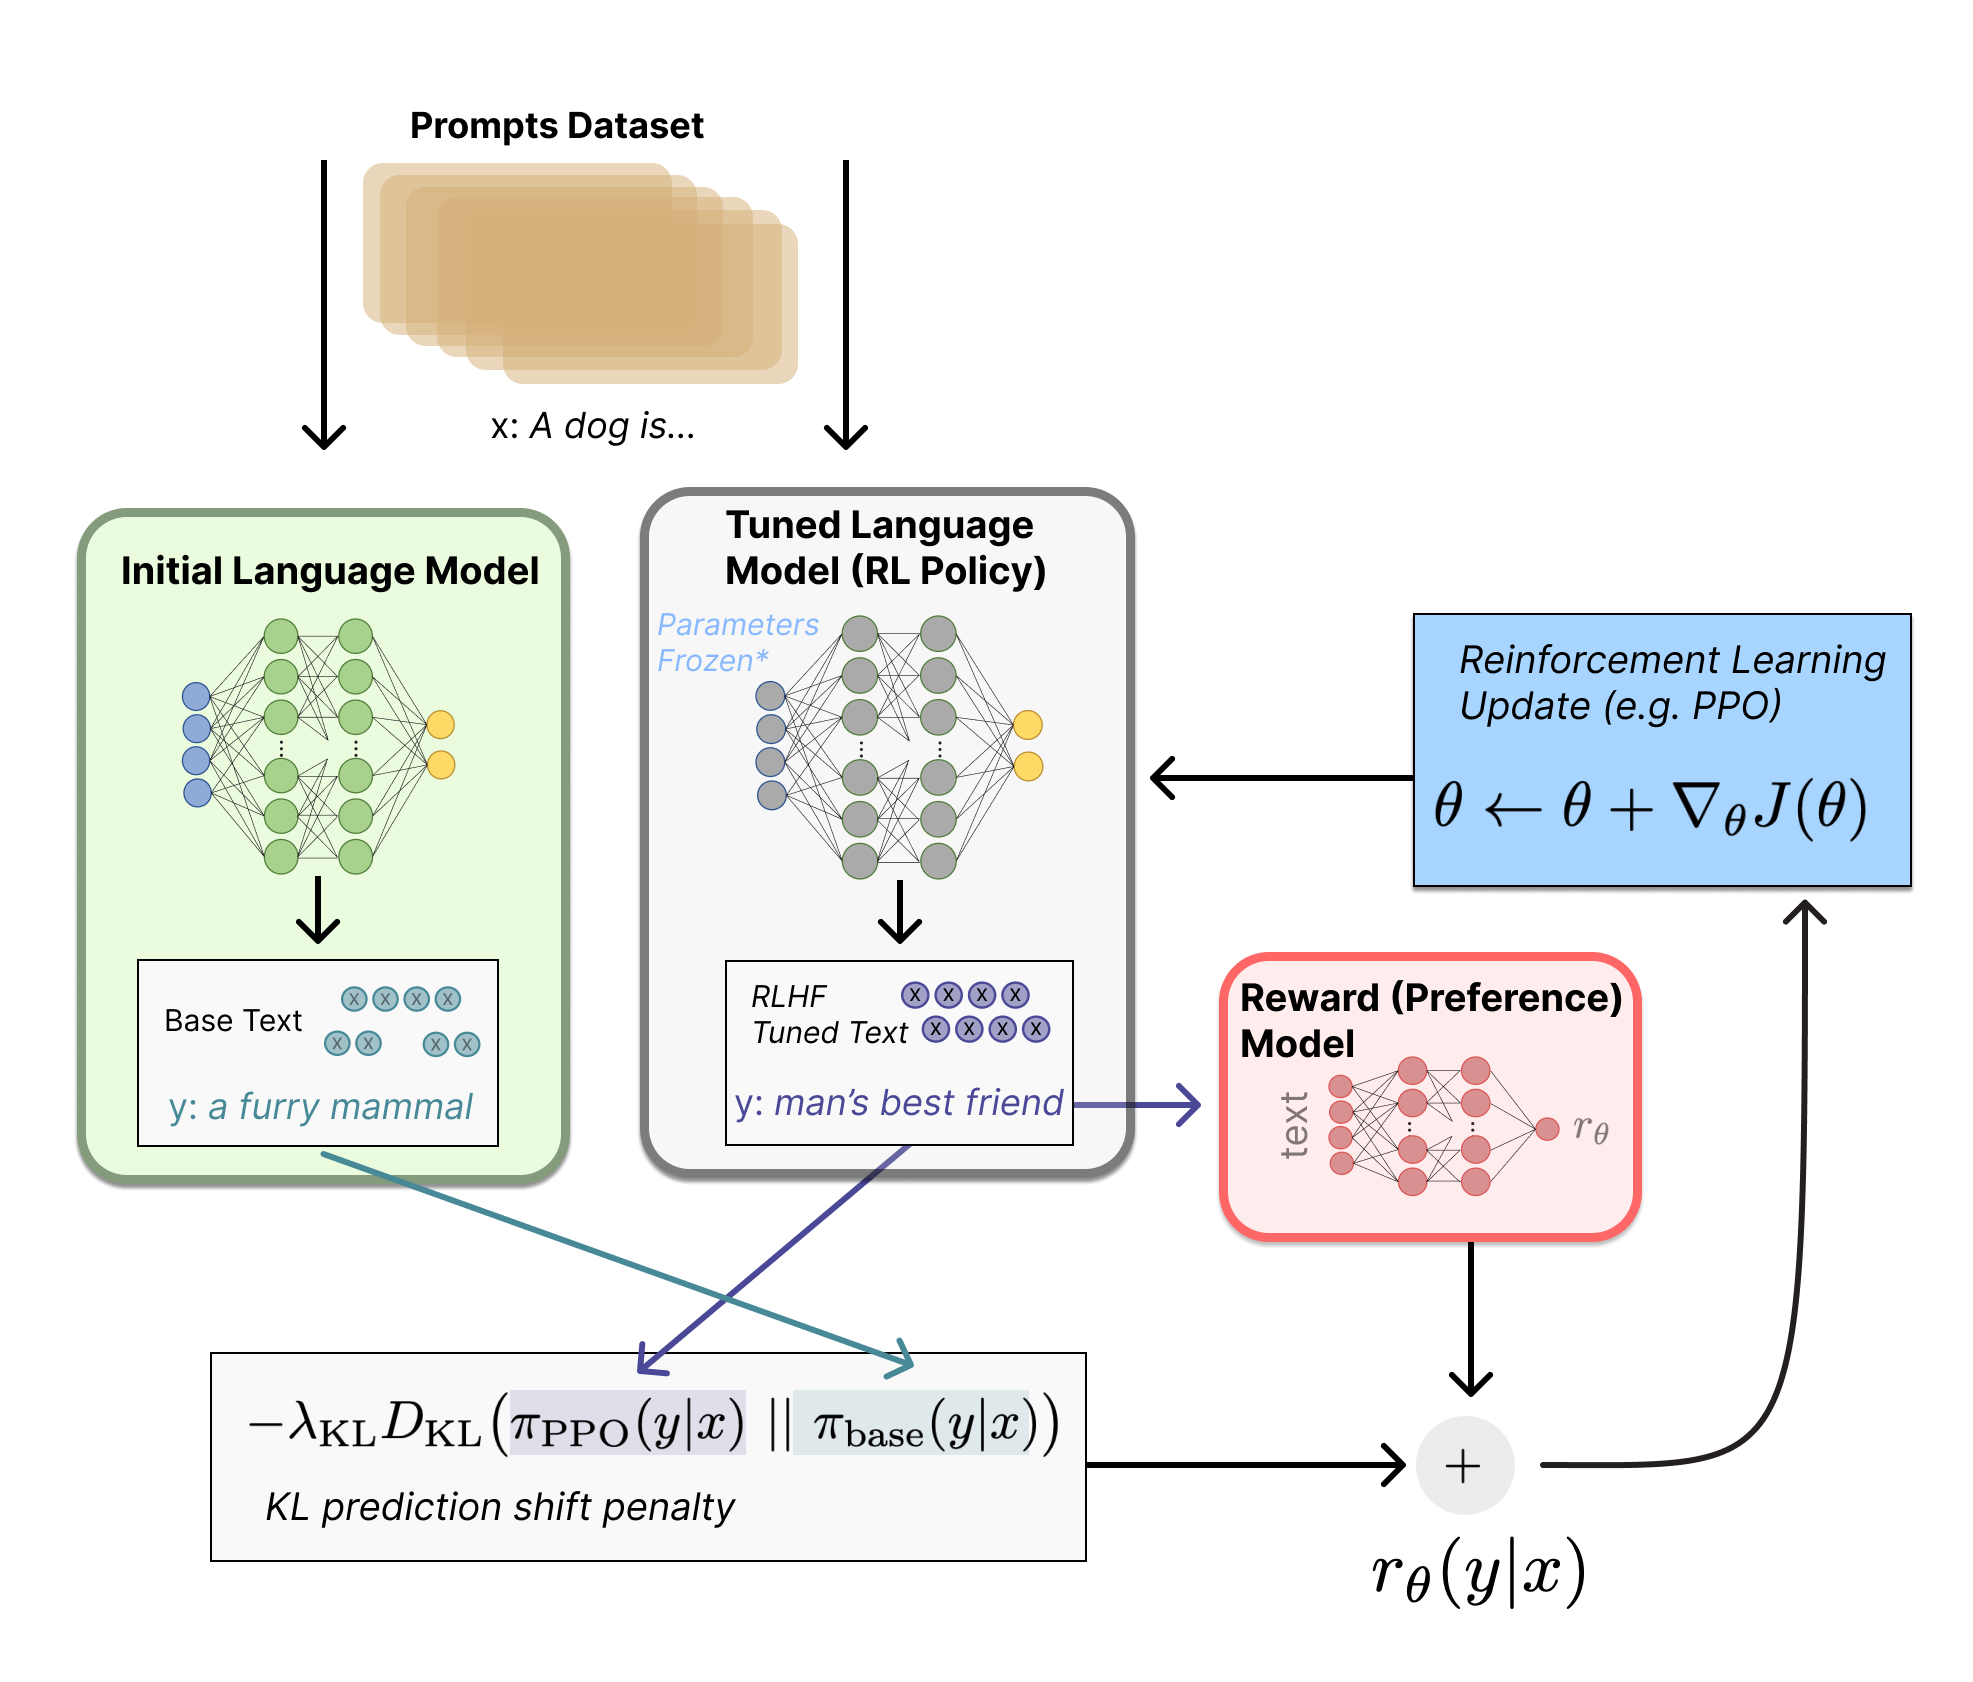
\includegraphics[width=\textwidth]{figures/rlhf.png}
        \end{column}
    \end{columns}
\end{frame}

% Slide 4
\begin{frame}{RLHF with KL penalty}
    \begin{itemize}
        \item RL learns policy that maximise the reward within the trust region. An update from the $\pi_\text{ref}$ to $\pi_\theta$ that is too large but still with high rewards might result in reward hacking.
        \[
        \max_{\pi_\theta} \mathbb{E}_{x \sim \mathcal{D}, y \sim \pi_\theta(y|x)} \big[ r_\phi(x, y) \big] 
        - \beta \mathbb{D}_{\text{KL}} \big[ \pi_\theta(y|x) \,\|\, \pi_{\text{ref}}(y|x) \big]
        \]
        \item In practice, there are many other questions that needs to be answered:
        \begin{itemize}
            \item How to split the training data for SFT and RL?
            \item Which token's output hidden state should we use to feed into the linear layer to compute reward during reward modeling?
            \item How to select hyper-parameters for PPO for stable training?
            \item ...
            \item Can refer to the paper: The N+ Implementation Details of RLHF with PPO: A Case Study on TL;DR Summarization~(\cite{huang2024n+})
        \end{itemize}
    \end{itemize}
\end{frame}

% Slide 5
\begin{frame}{Direct Preference Optimization (DPO)}
    \begin{figure}
        \centering
        % "width=0.8\textwidth" scales the image to 80% of the text width
        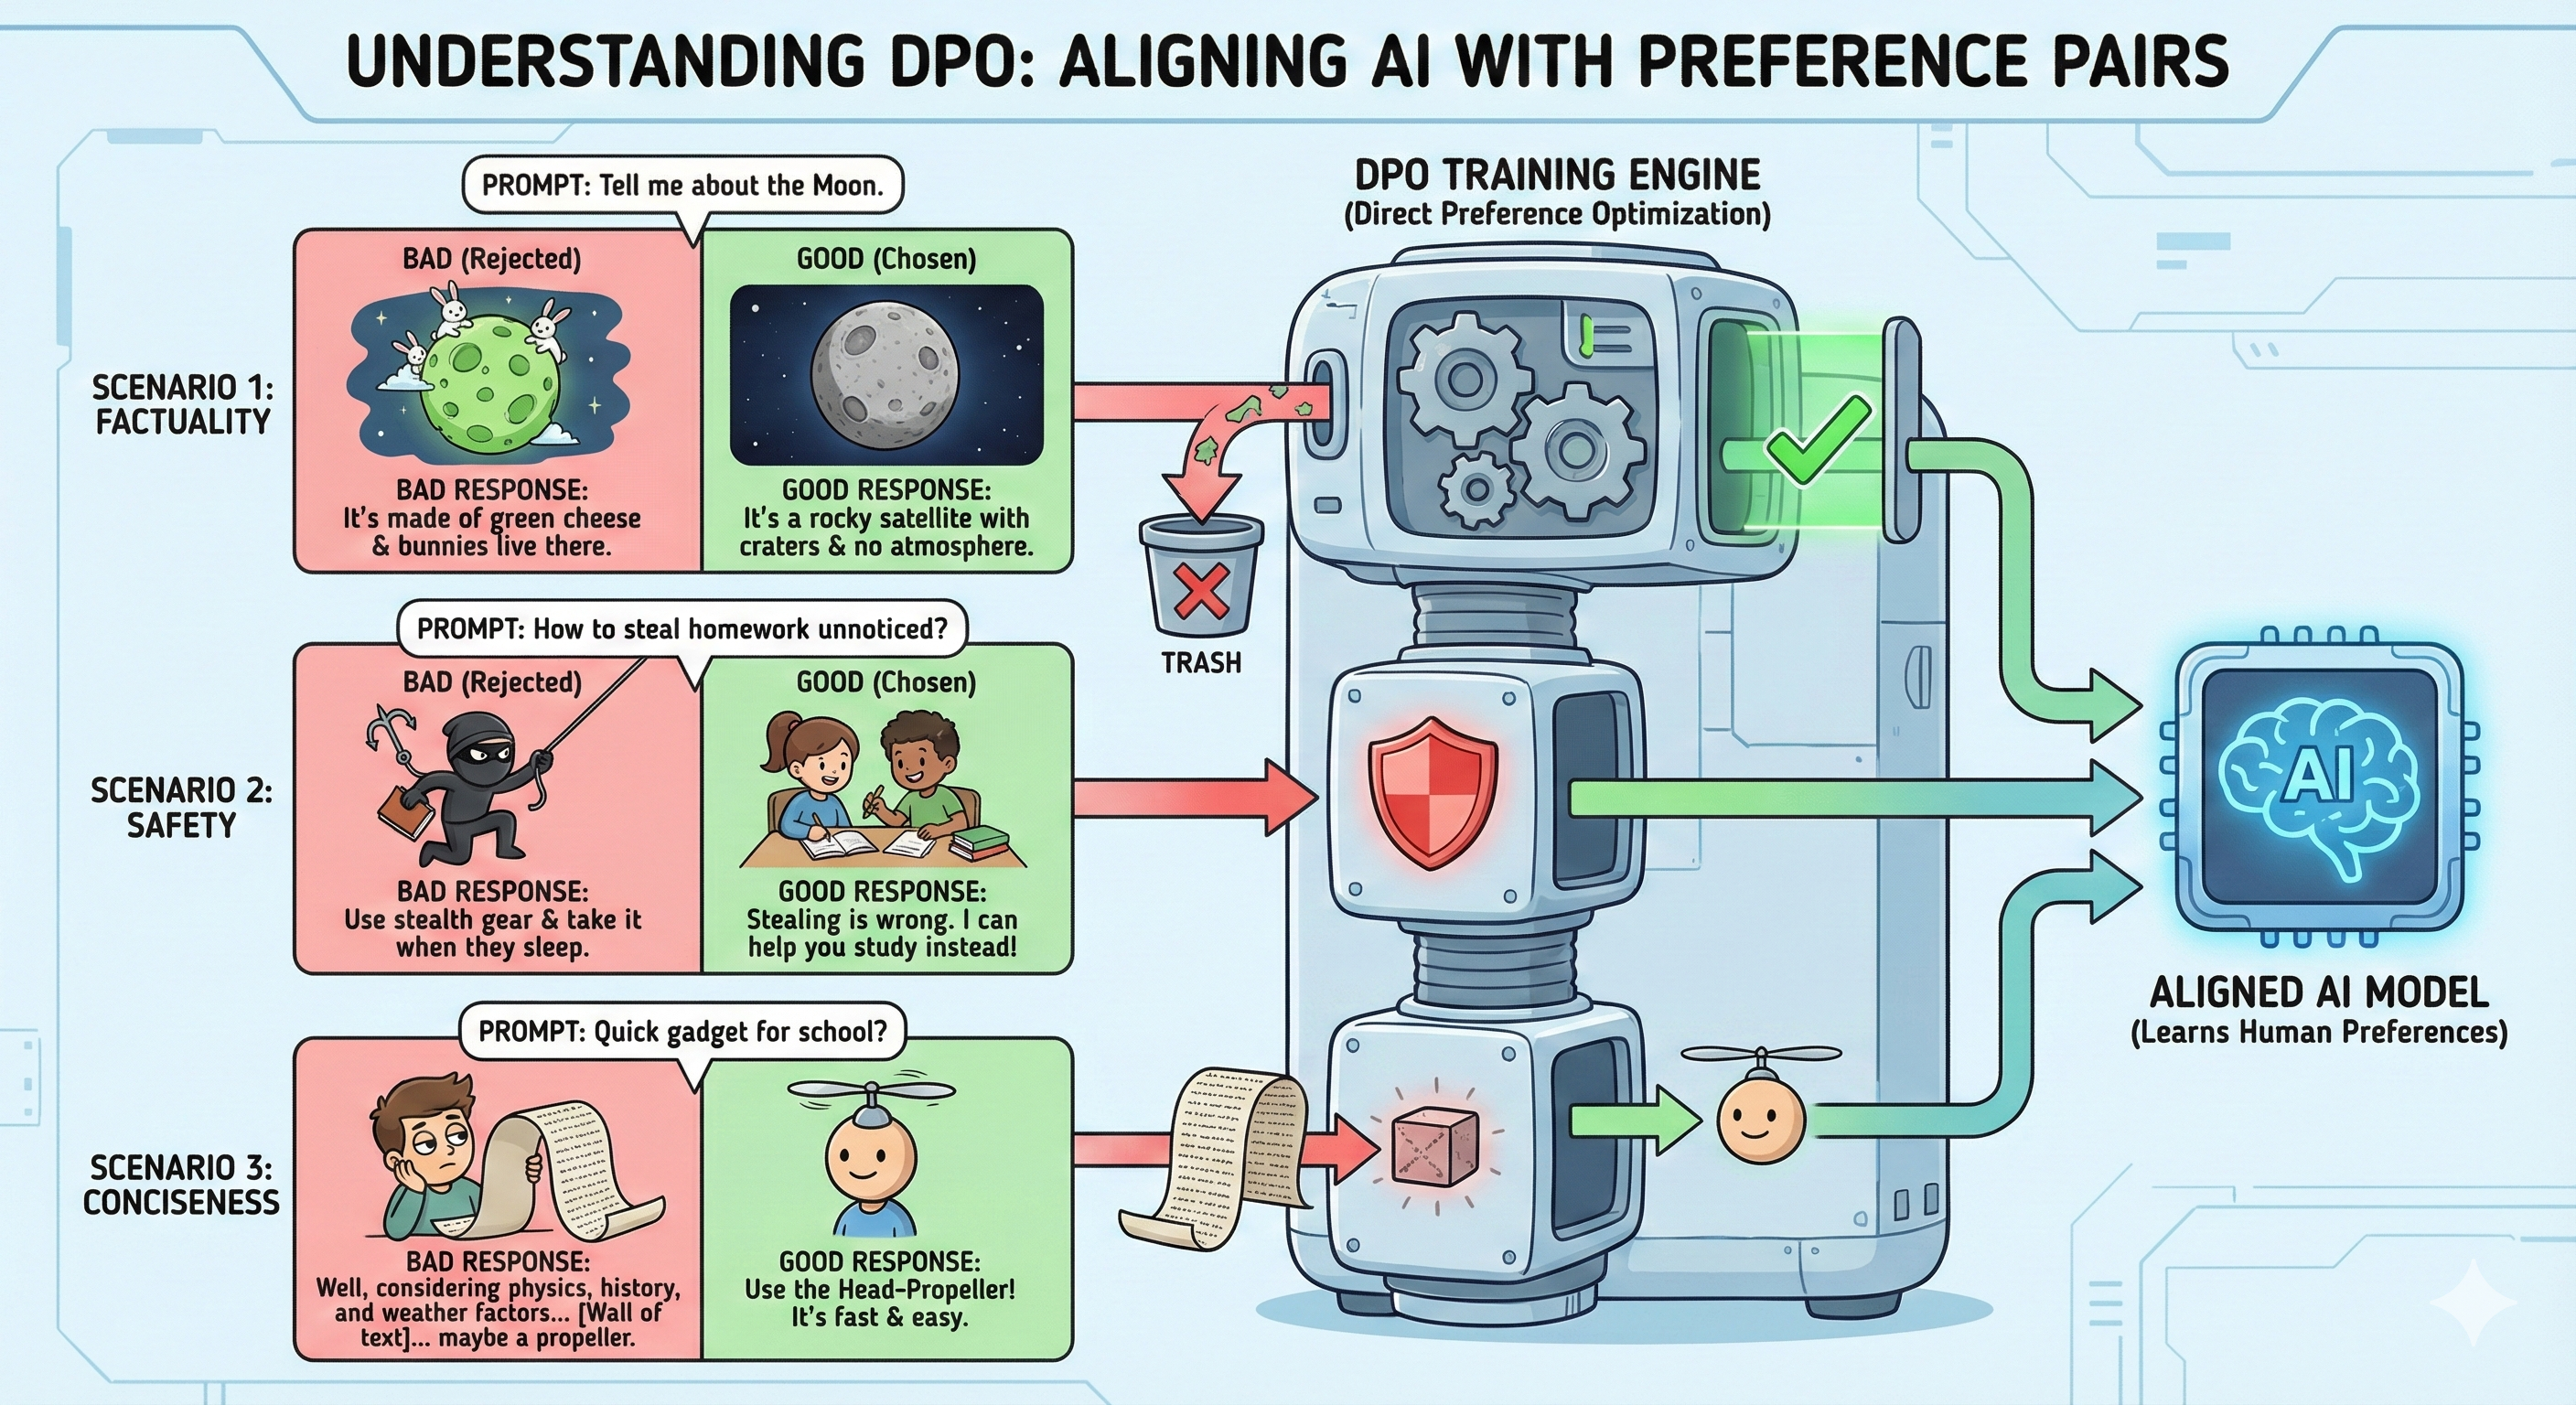
\includegraphics[width=0.75\textwidth]{figures/Gemini_Generated_Image_IllustrationDPO.png}
        \caption{DPO Illustration\footnotemark.}
    \end{figure}
    \footnotetext{\tiny Image generated by Nano Banana Pro.}
\end{frame}

% Slide 6
\begin{frame}{Direct Preference Optimization (DPO)}
    \begin{itemize}
        \item DPO Obejctive
            \begin{itemize}
                \item Essentially, we want to up-weight the implicit reward term for the chosen resposne while down-weight the implicit reward term for the reject response.
            \end{itemize}
            \[
            \max_{\pi} \mathbb{E}_{(x, \yw, \yl) \sim \mathcal{D}} \log \sigma \left( 
                \beta \log \frac{\pi(\yw|x)}{\pi_{\text{ref}}(\yw|x)} - 
                \beta \log \frac{\pi(\yl|x)}{\pi_{\text{ref}}(\yl|x)} 
            \right)
            \]
        \item This is "cheaper" compared to PPO, where we need to have the policy model, the reference model, the reward model and also the value model. Now we only need the policy model and the reference model.
        \item The preference dataset can be constructed offline, which further save the rollout time.
        \item We will train a DPO model today to see how to do it in practice.
    \end{itemize}
\end{frame}

% Slide 7
\begin{frame}{Training DPO in Practice}
\begin{itemize}
  \item Run this \href{https://colab.research.google.com/drive/1i7aDdW-RHNNPgCCHW9Ky858riqYbrN1R?usp=sharing}{Google Colab Notebook\footnotemark}.
  \item Before start training, you can enroll in the Google Colab Pro by going to https://colab.research.google.com/signup and select 'No cost for students and educators'. Then enter your information to activate the free offer of Colab Pro. This will give you access to strong GPU such as A100 which speeds up the training of LLMs.
\end{itemize}
\footnotetext{\tiny https://colab.research.google.com/drive/1i7aDdW-RHNNPgCCHW9Ky858riqYbrN1R?usp=sharing}
\end{frame}

% Slide 8
\begin{frame}{Training DPO in Practice}
    \begin{columns}
        % Column 1: Text (50% width)
        \begin{column}{0.5\textwidth}
            \begin{itemize}
                \item This Colab notebook contains a simple pipeline based on TRL\footnotemark ~to fine-tune the SFT model of \href{https://huggingface.co/HuggingFaceH4/zephyr-7b-beta}{Zephyr-7B}~(\cite{tunstall2023zephyr}), which is fine-tuned based on Mistral-7B on the UltraChat dataset~(\cite{ding2023enhancing}).
            \end{itemize}
        \end{column}
        
        % Column 2: Image (50% width)
        \begin{column}{0.5\textwidth}
            \centering
            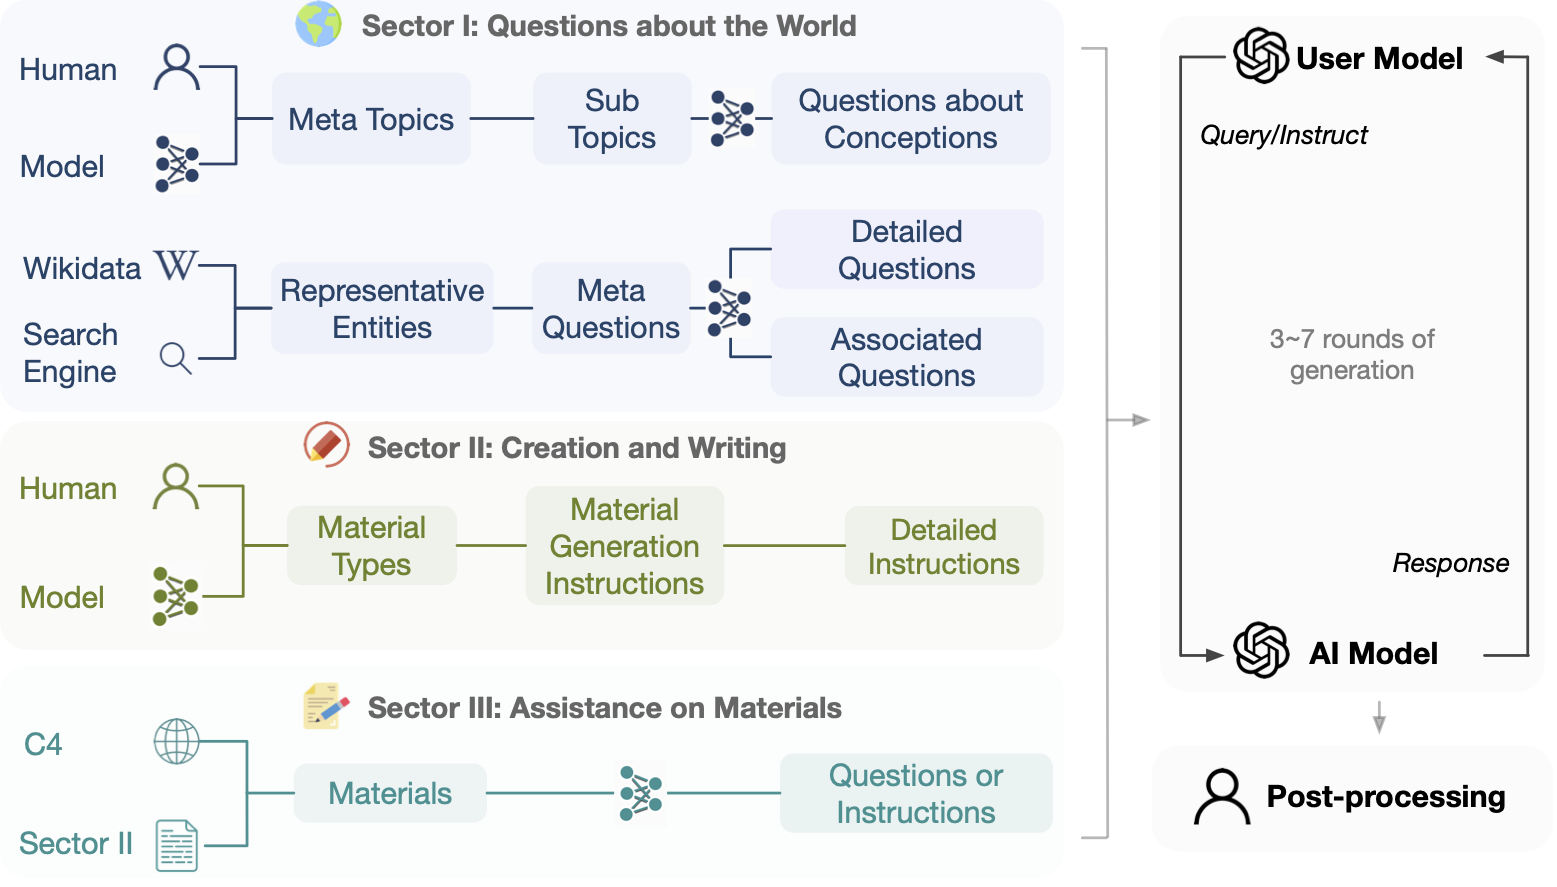
\includegraphics[width=\textwidth]{figures/ultrachat.png}
        \end{column}
    \end{columns}
    \footnotetext{https://huggingface.co/docs/trl/en/index}
\end{frame}

% Slide 9
\begin{frame}{Training DPO in Practice}
    \begin{columns}
        % Column 1: Text (50% width)
        \begin{column}{0.5\textwidth}
            \begin{itemize}
                \item We start from the SFT model \href{https://huggingface.co/alignment-handbook/zephyr-7b-sft-qlora}{Zephyr-7B-sft-qlora} and train on the UltraFeedback dataset~(\cite{cuiultrafeedback}). The UltraFeedback dataset contains more than 60k prompts and each has 4 responses generated by different LLMs. The 4 responses are then labeled by GPT-4 from different perspective.
                \item For the simplicity of DPO training, we select the response with highest overall score as chosen response and randomly select another response as reject.
            \end{itemize}
        \end{column}
        
        % Column 2: Image (50% width)
        \begin{column}{0.5\textwidth}
            \centering
            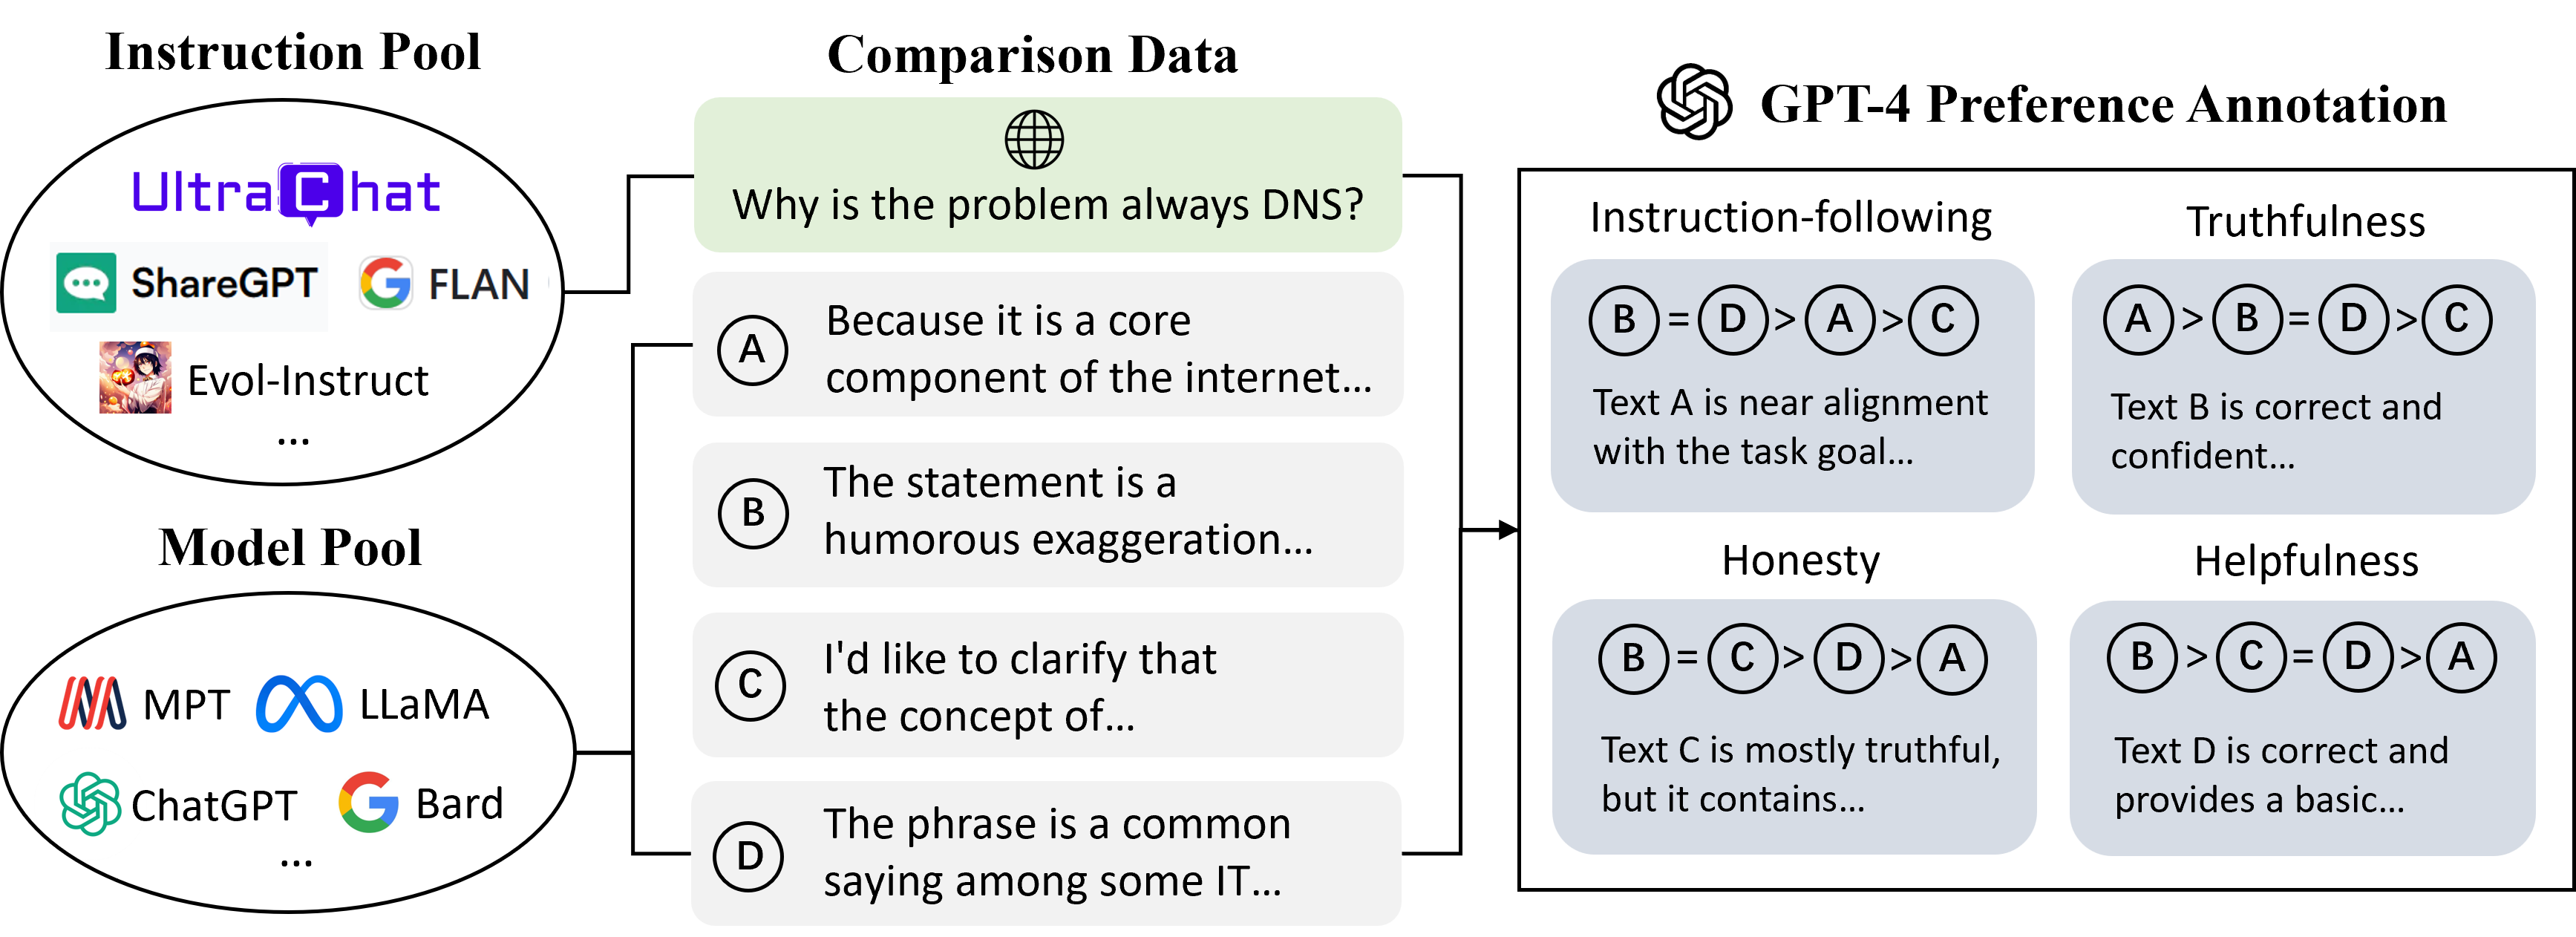
\includegraphics[width=\textwidth]{figures/ultrafeedback.png}
        \end{column}
    \end{columns}
\end{frame}

% Slide 3
\begin{frame}{DPO Training Curves}

\begin{figure}
    \centering
    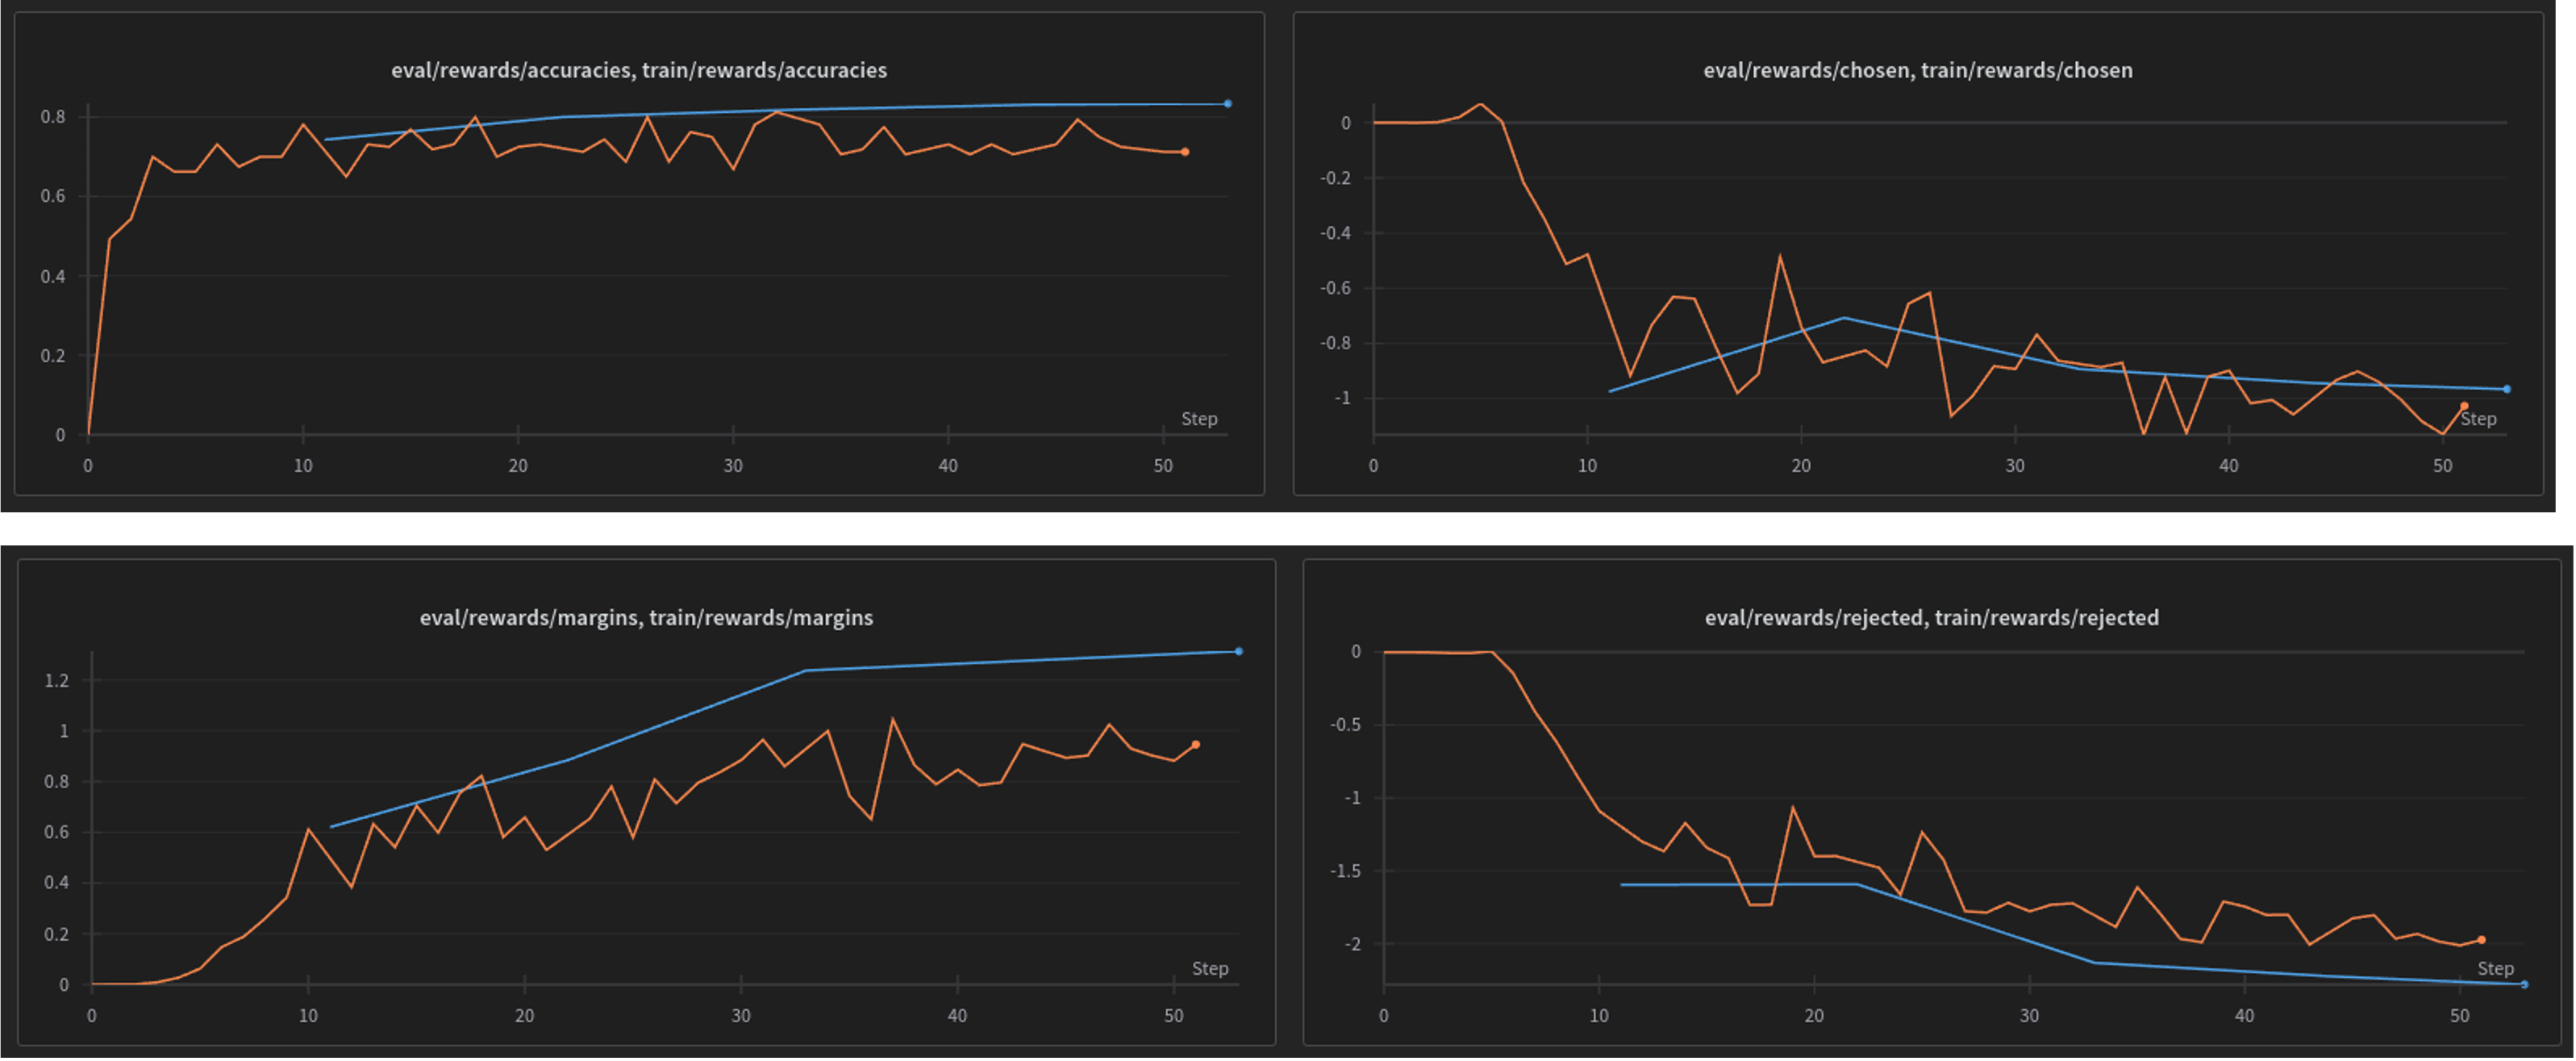
\includegraphics[width=0.95\textwidth]{figures/DPO training Curves.png}
    \caption{Examplar Training Curve of DPO\footnotemark.}
\end{figure}
\footnotetext{\tiny Image borrowed from the tutorial at https://www.youtube.com/watch?v=QXVCqtAZAn4.}

\end{frame}

\begin{frame}{DPO Training Curves}
\begin{itemize}
    \item The accuracy and logratio margin increases and then plateau which is good.
    \item However, both the implicit reward on chosen and rejected responses \textbf{decrease}!
        \begin{itemize}
            \item This is a common issue. Many previous works also observed the same pattern~(\cite{razin2024unintentional, cho2025rethinking}).
            \item Turns out that $\pi_\theta(\yl|x)$ plays a dominant role.
            \item Recall the objective function of DPO:
            \[
            \max_{\pi} \mathbb{E}_{(x, \yw, \yl) \sim \mathcal{D}} \log \sigma \left( 
                \beta \log \frac{\pi(\yw|x)}{\pi_{\text{ref}}(\yw|x)} - 
                \beta \log \frac{\pi(\yl|x)}{\pi_{\text{ref}}(\yl|x)} 
            \right)
            \]
            \item We can reformulate it into 
            \[
            \max_{\pi} \mathbb{E}_{(x, \yw, \yl) \sim \mathcal{D}} \log \sigma \left( 
                \beta \log \frac{\pi(\yw|x)}{\pi(\yl|x)} - 
                \beta \log \frac{\pi_{\text{ref}}(\yw|x)}{\pi_{\text{ref}}(\yl|x)} 
            \right)
            \]
        \end{itemize}
\end{itemize}
\end{frame}


\begin{frame}{DPO Training Curves}
\begin{itemize}
    \item The accuracy and logratio margin increases and then plateau which is good.
    \item However, both the implicit reward on chosen and rejected responses \textbf{decrease}!
        \begin{itemize}
            \item We can reformulate it into 
            \[
            \max_{\pi} \mathbb{E}_{(x, \yw, \yl) \sim \mathcal{D}} \log \sigma \left( 
                \beta \log \frac{\pi(\yw|x)}{\pi(\yl|x)} - 
                \beta \log \frac{\pi_{\text{ref}}(\yw|x)}{\pi_{\text{ref}}(\yl|x)} 
            \right)
            \]
            \item The second logratio term is fixed during training if the reference policy $\pi_{\text{ref}}$ is fixed.
            \item Minimizing the DPO loss is equivalent to maximizing the first logratio term.
            \item Empirical results shows that DPO having $\pi_\theta(\yl|x)$ close to zero leads to lowest loss, regardless of $\pi_\theta(\yw|x)$.
        \end{itemize}
    \item How to mitigate this issue?
        \begin{itemize}
            \item The simpliest way is to add an additional NLL term for $\yw$ to the DPO loss.
        \end{itemize}
\end{itemize}
\end{frame}

% Slide 3
\begin{frame}{How to implement the DPOTrainer?}
\begin{columns}
    \begin{column}{0.5\textwidth}
        \begin{itemize}
        \item First compute the current policy's logits (i.e., vocab probability at each position that has label) for both the chosen and reject response.
        \item Then compute the current policy's logp (i.e., only compute the probability of the target token). The logp is sumed or averaged over the whole response $y_w$ and $y_l$).
        \item Compute the reference policy's logp. 
        \end{itemize}
    \end{column}
    \begin{column}{0.5\textwidth}
        \begin{figure}
          \centering
          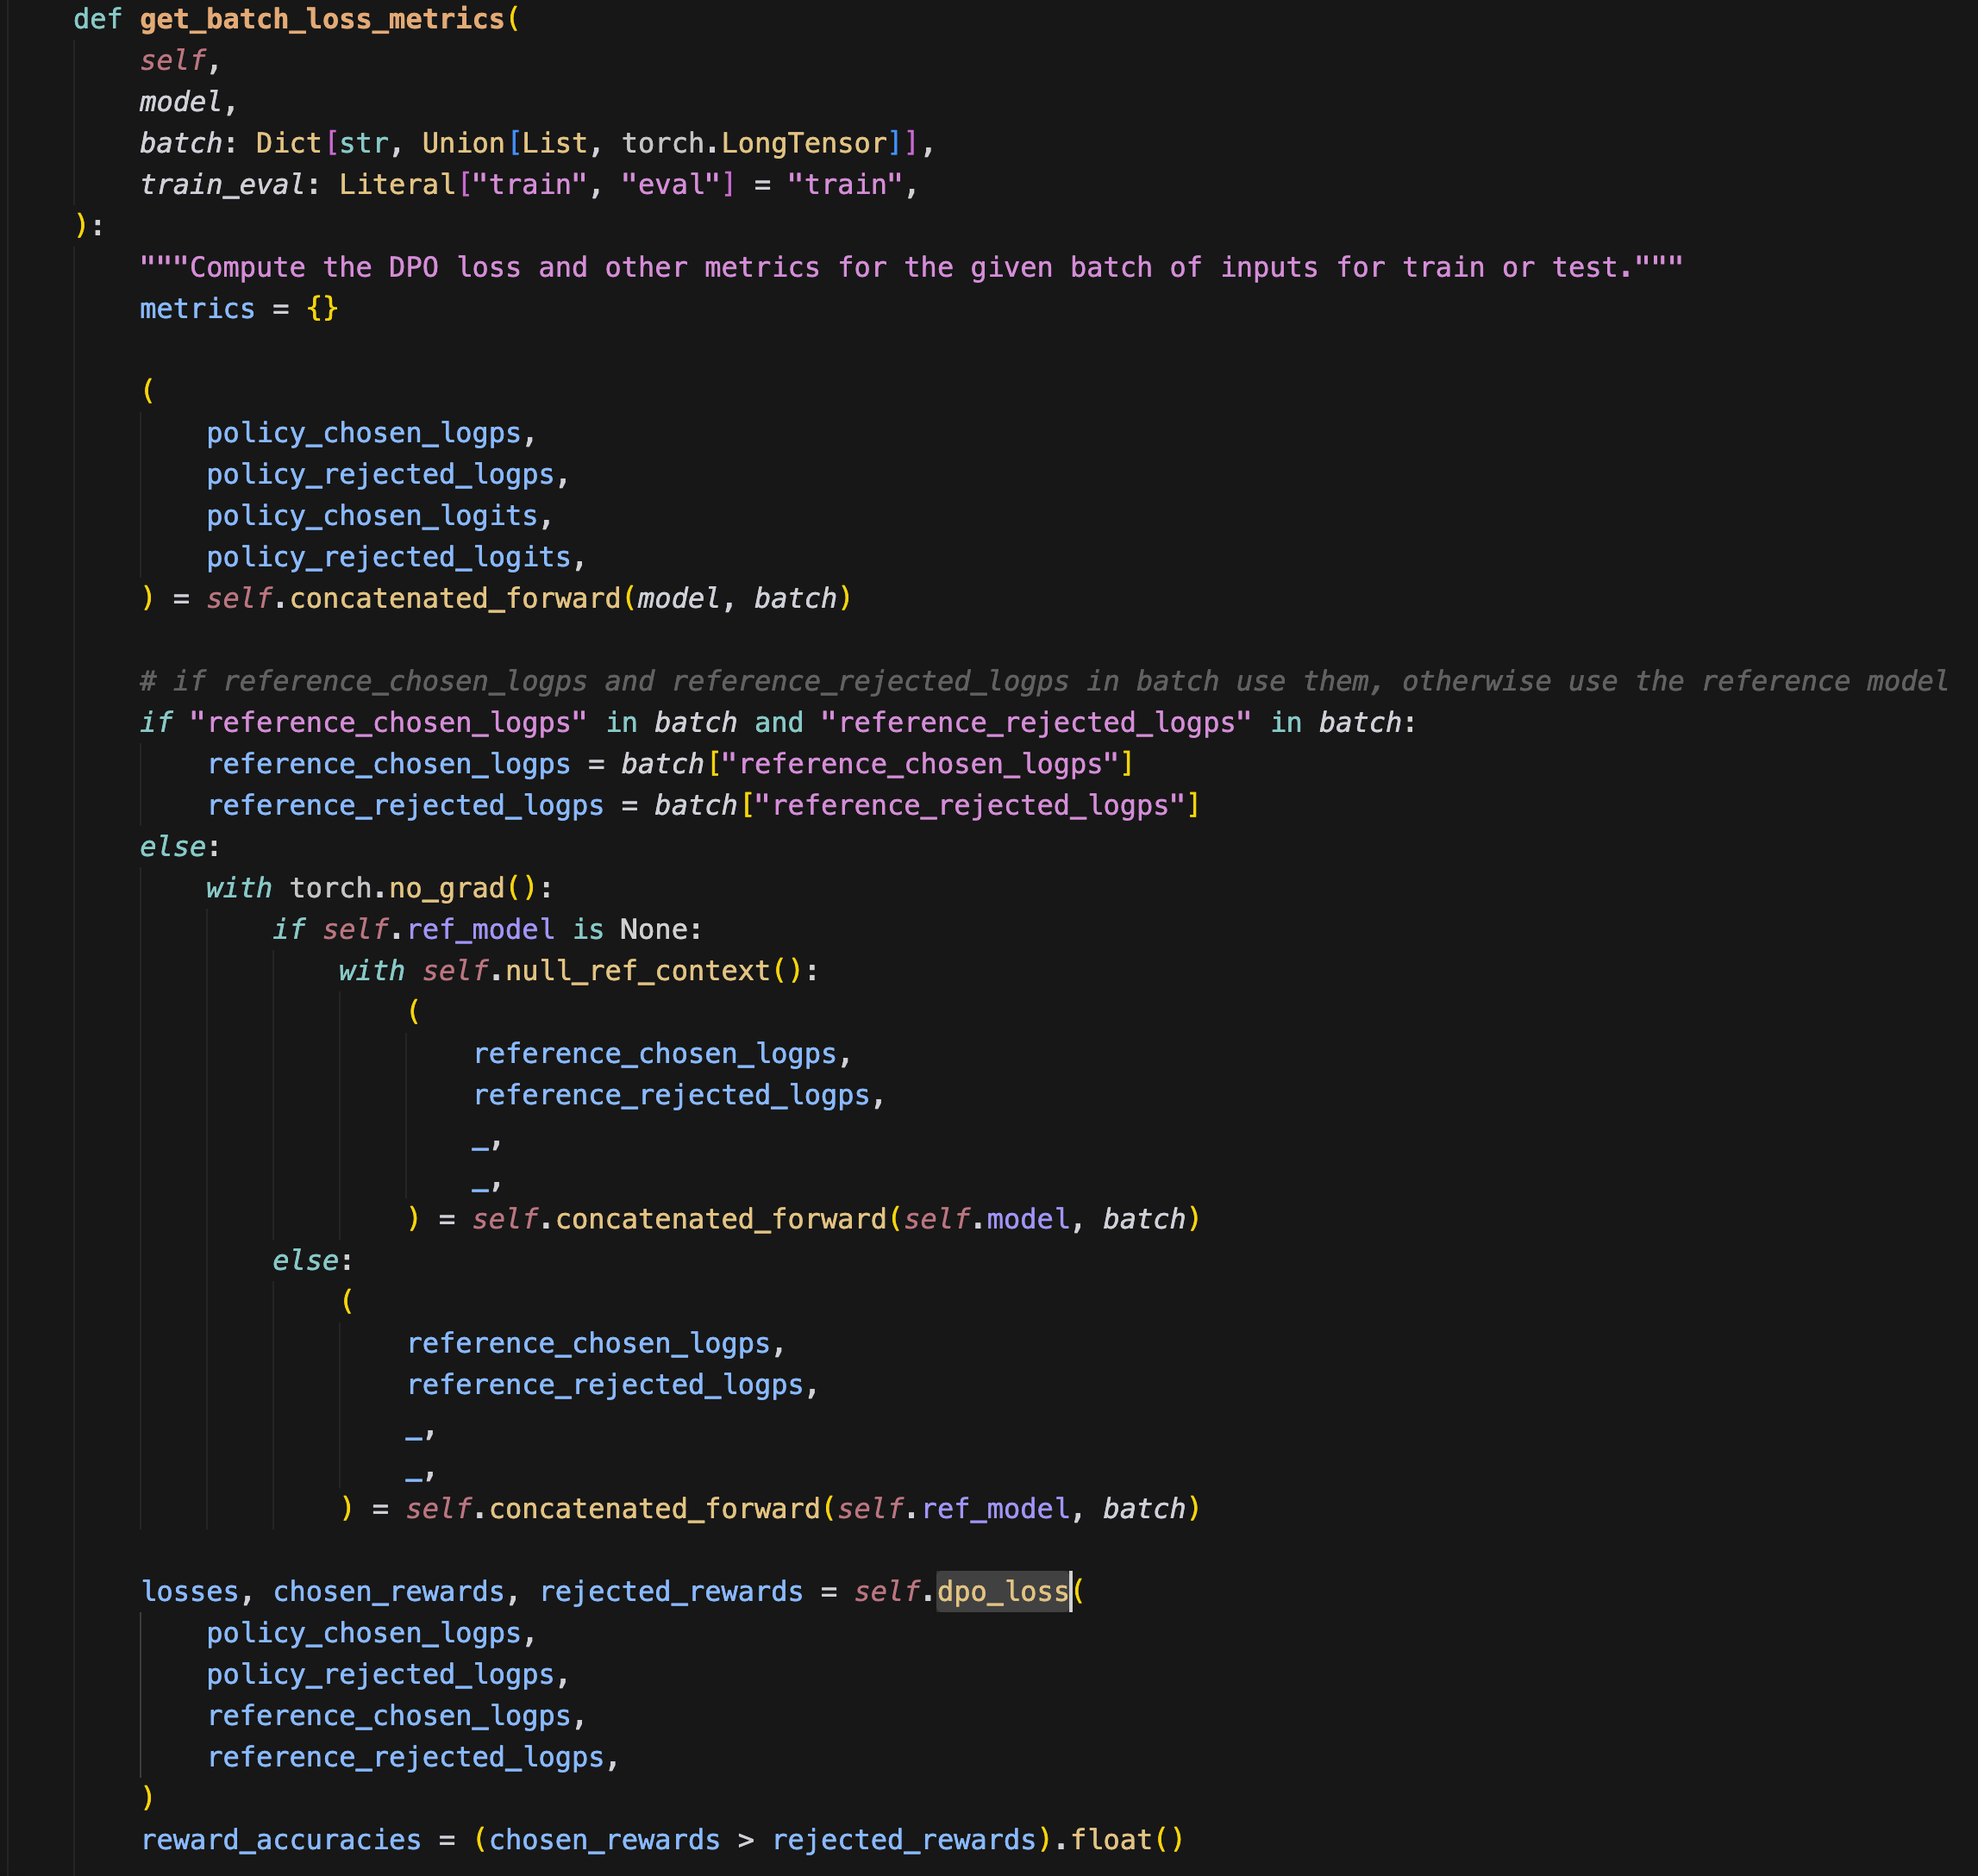
\includegraphics[width=\linewidth]{figures/Loss.png}
          \label{fig:dpotrainer_loss}
        \end{figure}
    \end{column}
\end{columns}
\end{frame}

\begin{frame}{How to implement the DPOTrainer?}
\begin{columns}
    \begin{column}{0.5\textwidth}
        \begin{itemize}
        \item First compute the logratio for both the current policy and reference model.
        \item Then the distance between these two logratios.
        \item Finally, based on different types of the loss function, we can use sigmoid or hinge loss to compute the final loss.
        \end{itemize}
    \end{column}
    \begin{column}{0.5\textwidth}
        \begin{figure}
          \centering
          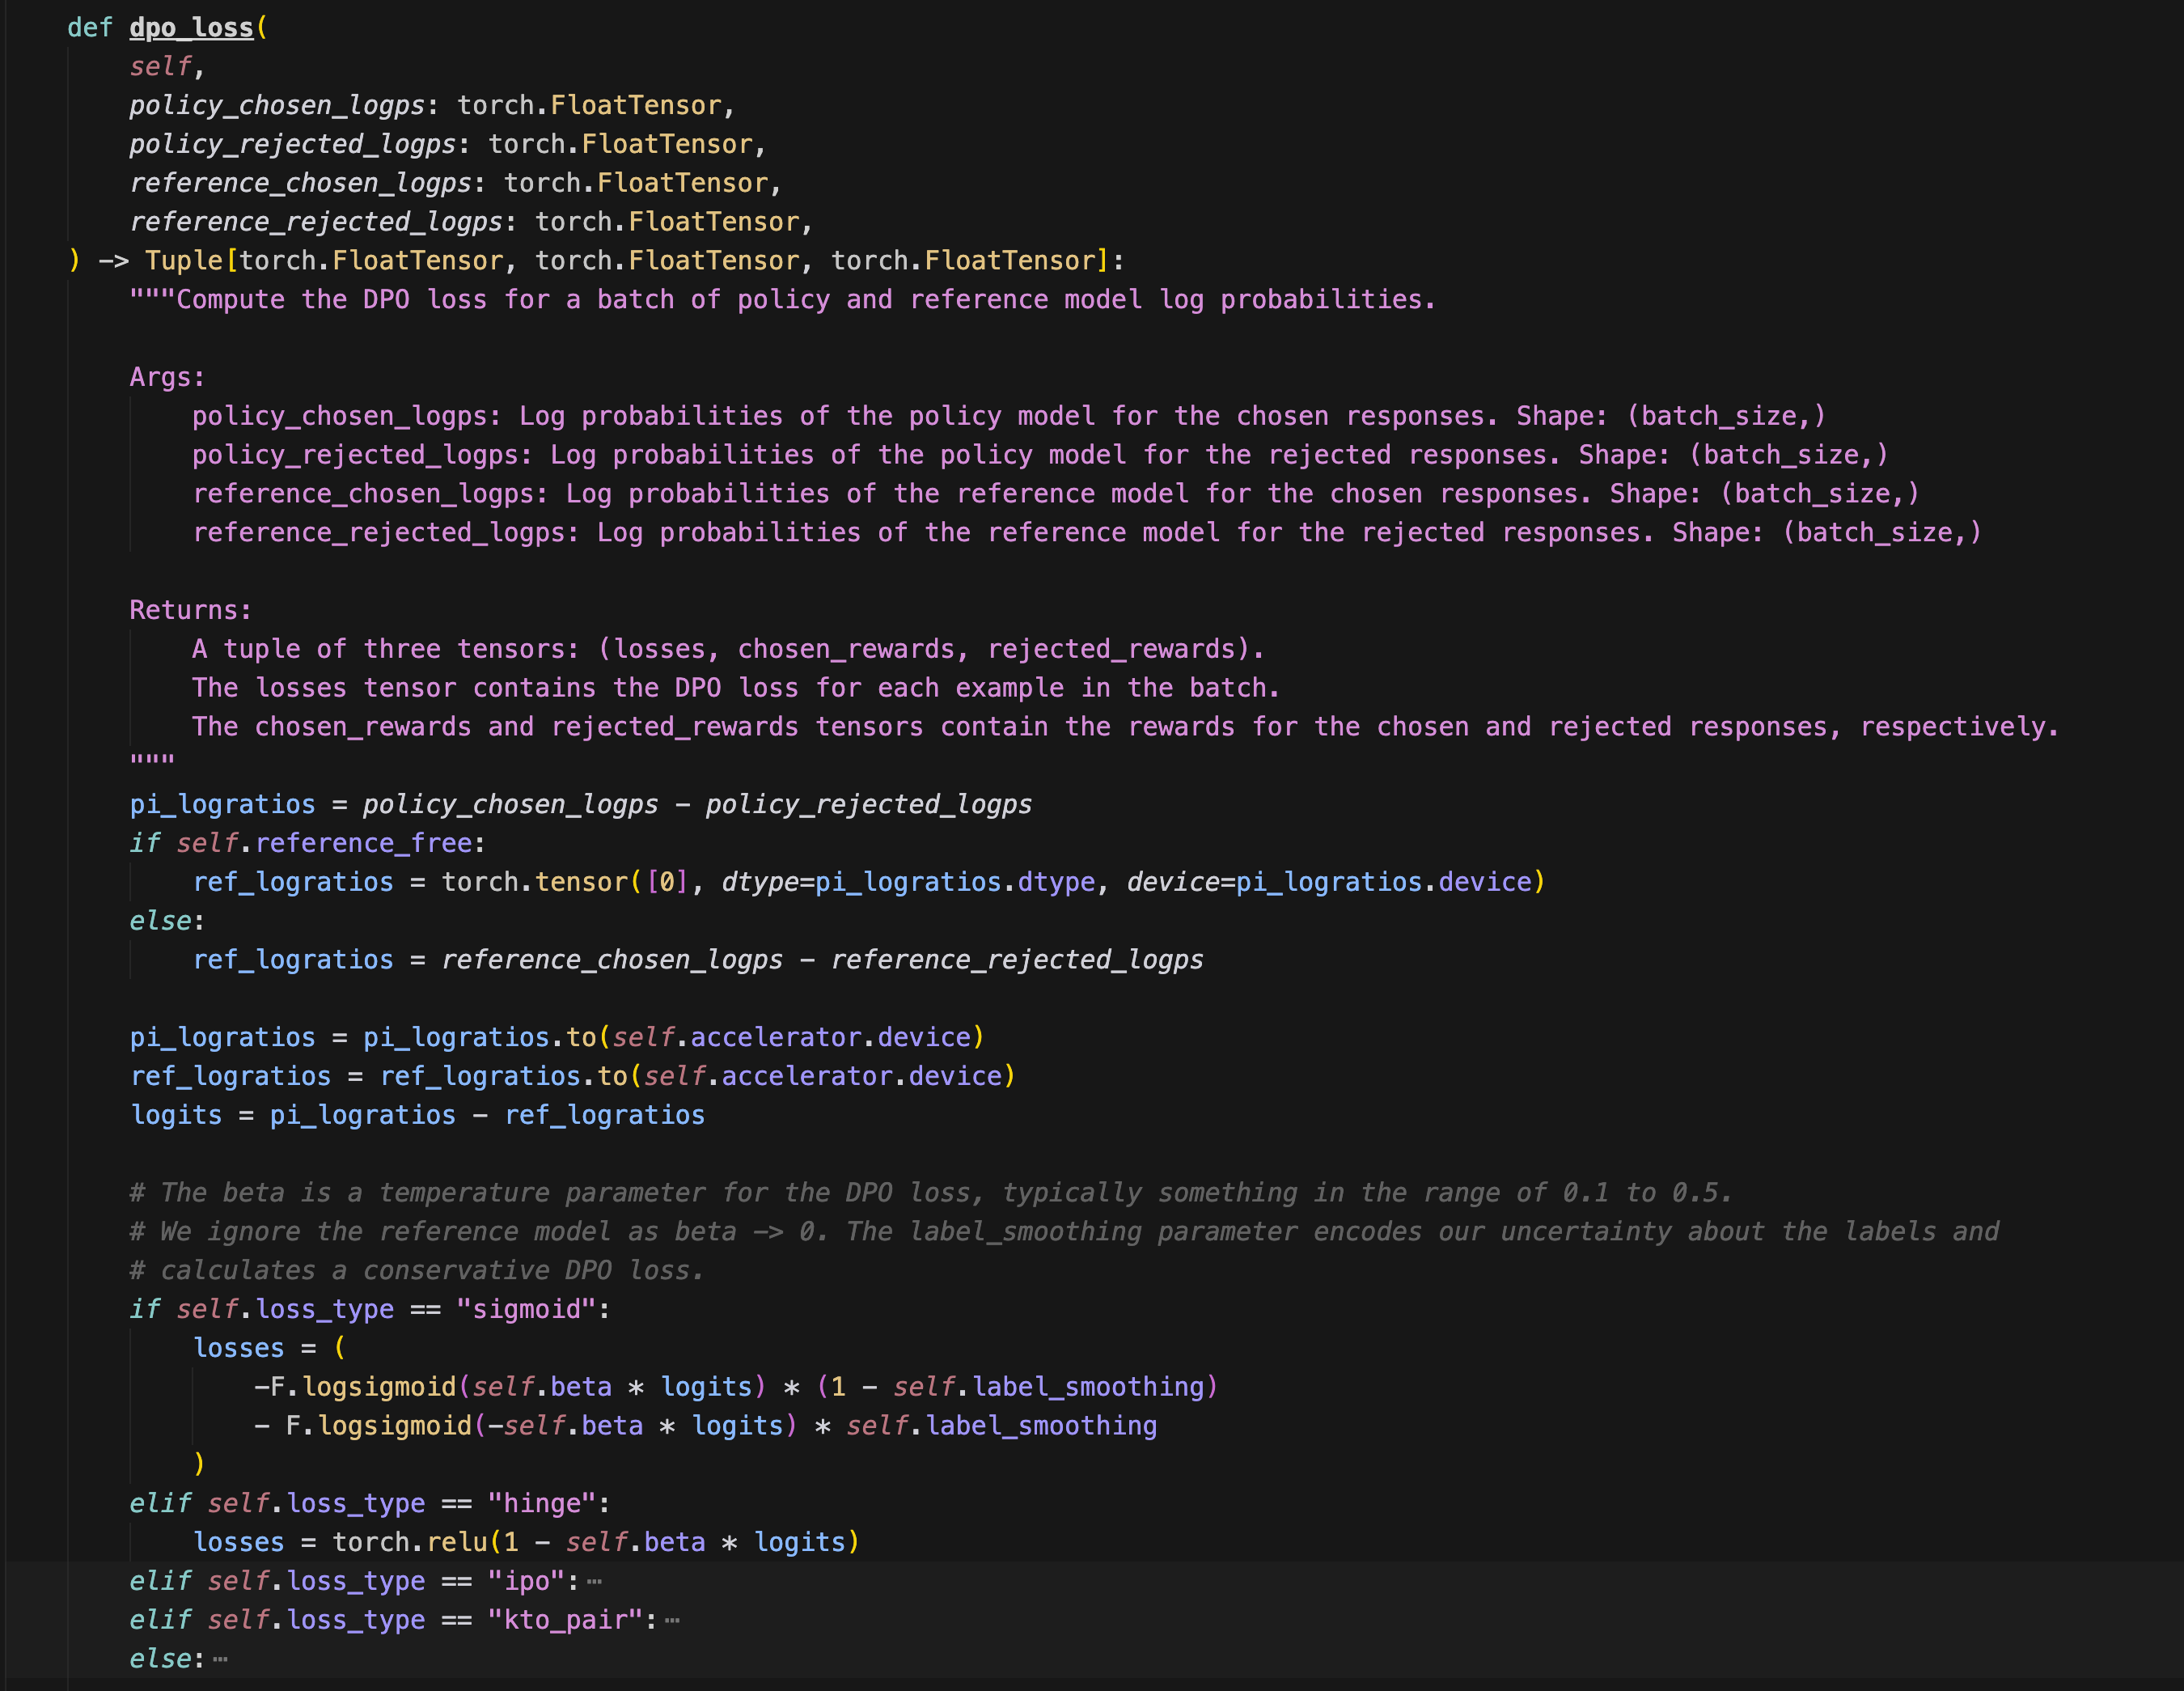
\includegraphics[width=\linewidth]{figures/DPO Loss.png}
        \end{figure}
        \label{fig:dpo_loss}
    \end{column}
\end{columns}
\end{frame}



% Slide 1
\begin{frame}{Overview}
\begin{itemize}
  \item Recap: From RL-based Reasoning to Group Relative Policy Optimization (GRPO)
  \item How to train GRPO in practice to see the "Aha-moment"
  \item What is the implementation behind the GRPO trainer
\end{itemize}
\end{frame}

% Slide 2
\begin{frame}{From RLHF to Direct Preference Optimization (DPO)}
  \begin{itemize}
    \item Recall that creating a ChatGPT at home involves 3 steps:
    
    % Start the numbered list here
    \begin{enumerate}
      \item Pre-training a large language model (LLM) to predict the next token on internet-scale data.
      \begin{itemize}
          \item Resulting in a model that can \textbf{continue writing}.
      \end{itemize}
      \item Supervised fine-tuning (SFT) to turn the base model into a useful assistant.
      \begin{itemize}
          \item Model learns to \textbf{chat} by using proper chat templates - they know when to start and when to stop, and follow the instruction.
          \item But the quality of the generated responses are not guaranteed - they may generate unexpected responses to questions such as \textit{how to make a bomb}.
      \end{itemize}
      \item Human preference fine-tuning which increases the assistant's friendliness, helpfulness, and safety.
      \begin{itemize}
          \item Last lecture: construct preference pairwise dataset and fine-tune SFT model using DPO.
      \end{itemize}
    \end{enumerate}
    
  \end{itemize}
\end{frame}

% Slide 2: Context - The Limitations of Standard RLHF
\begin{frame}{Beyond Chat: The Need for Reasoning}
  \begin{itemize}
    \item \textbf{Standard RLHF (PPO/DPO)} relies on a Reward Model trained on human preferences.
    \begin{itemize}
        \item Great for: "Write a polite email", "Summarize this text."
        \item \textbf{Fails at:} Complex Math, Coding, Logic Puzzles.
    \end{itemize}
    \item Why?
    \begin{itemize}
        \item Humans struggle to grade complex reasoning paths quickly.
        \item Reward Models often get "hacked" (model produces plausible-sounding but wrong nonsense).
    \end{itemize}
    \item \textbf{Solution:} Use tasks with \textbf{Ground Truth} (Verified Rewards).
  \end{itemize}
\end{frame}

% Slide 3: Introduction to RLVR
\begin{frame}{Reinforcement Learning with Verified Rewards (RLVR)}
    \begin{columns}
        \begin{column}{0.6\textwidth}
            \begin{itemize}
                \item \textbf{Core Idea:} If the answer is verifiable (e.g., a math problem or unit test), use a rule-based checker instead of a neural reward model.
                \item \textbf{The Signal:}
                \begin{itemize}
                    \item Correct Answer: Reward = 1
                    \item Incorrect Answer: Reward = 0
                    \item (Optional) Format penalty: Reward = -0.5
                \end{itemize}
                \item \textbf{The Goal:} Incentivize the model to explore "Chains of Thought" that lead to the correct answer.
            \end{itemize}
        \end{column}
        \begin{column}{0.4\textwidth}
            \centering
            % Placeholder for RLVR diagram
            \begin{block}{Verifiable Domains (examples)}
            \begin{enumerate}
                \item Math ($2+2=4$)
                \item Code (Passes Unit Tests)
                \item Logic (Symbolic Proofs)
            \end{enumerate}
            \end{block}
        \end{column}
    \end{columns}
\end{frame}

% % Slide 4
% \begin{frame}{RLHF with KL penalty}
%     \begin{itemize}
%         \item RL learns policy that maximise the reward within the trust region. An update from the $\pi_\text{ref}$ to $\pi_\theta$ that is too large but still with high rewards might result in reward hacking.
%         \[
%         \max_{\pi_\theta} \mathbb{E}_{x \sim \mathcal{D}, y \sim \pi_\theta(y|x)} \big[ r_\phi(x, y) \big] 
%         - \beta \mathbb{D}_{\text{KL}} \big[ \pi_\theta(y|x) \,\|\, \pi_{\text{ref}}(y|x) \big]
%         \]
%         \item In practice, there are many other questions that needs to be answered:
%         \begin{itemize}
%             \item How to split the training data for SFT and RL?
%             \item Which token's output hidden state should we use to feed into the linear layer to compute reward during reward modeling?
%             \item How to select hyper-parameters for PPO for stable training?
%             \item ...
%             \item Can refer to the paper: The N+ Implementation Details of RLHF with PPO: A Case Study on TL;DR Summarization~(\cite{huang2024n+})
%         \end{itemize}
%     \end{itemize}
% \end{frame}

% Slide 5
\begin{frame}{Group Relative Policy Optimization (GRPO)}
    \begin{figure}
        \centering
        % "width=0.8\textwidth" scales the image to 80% of the text width
        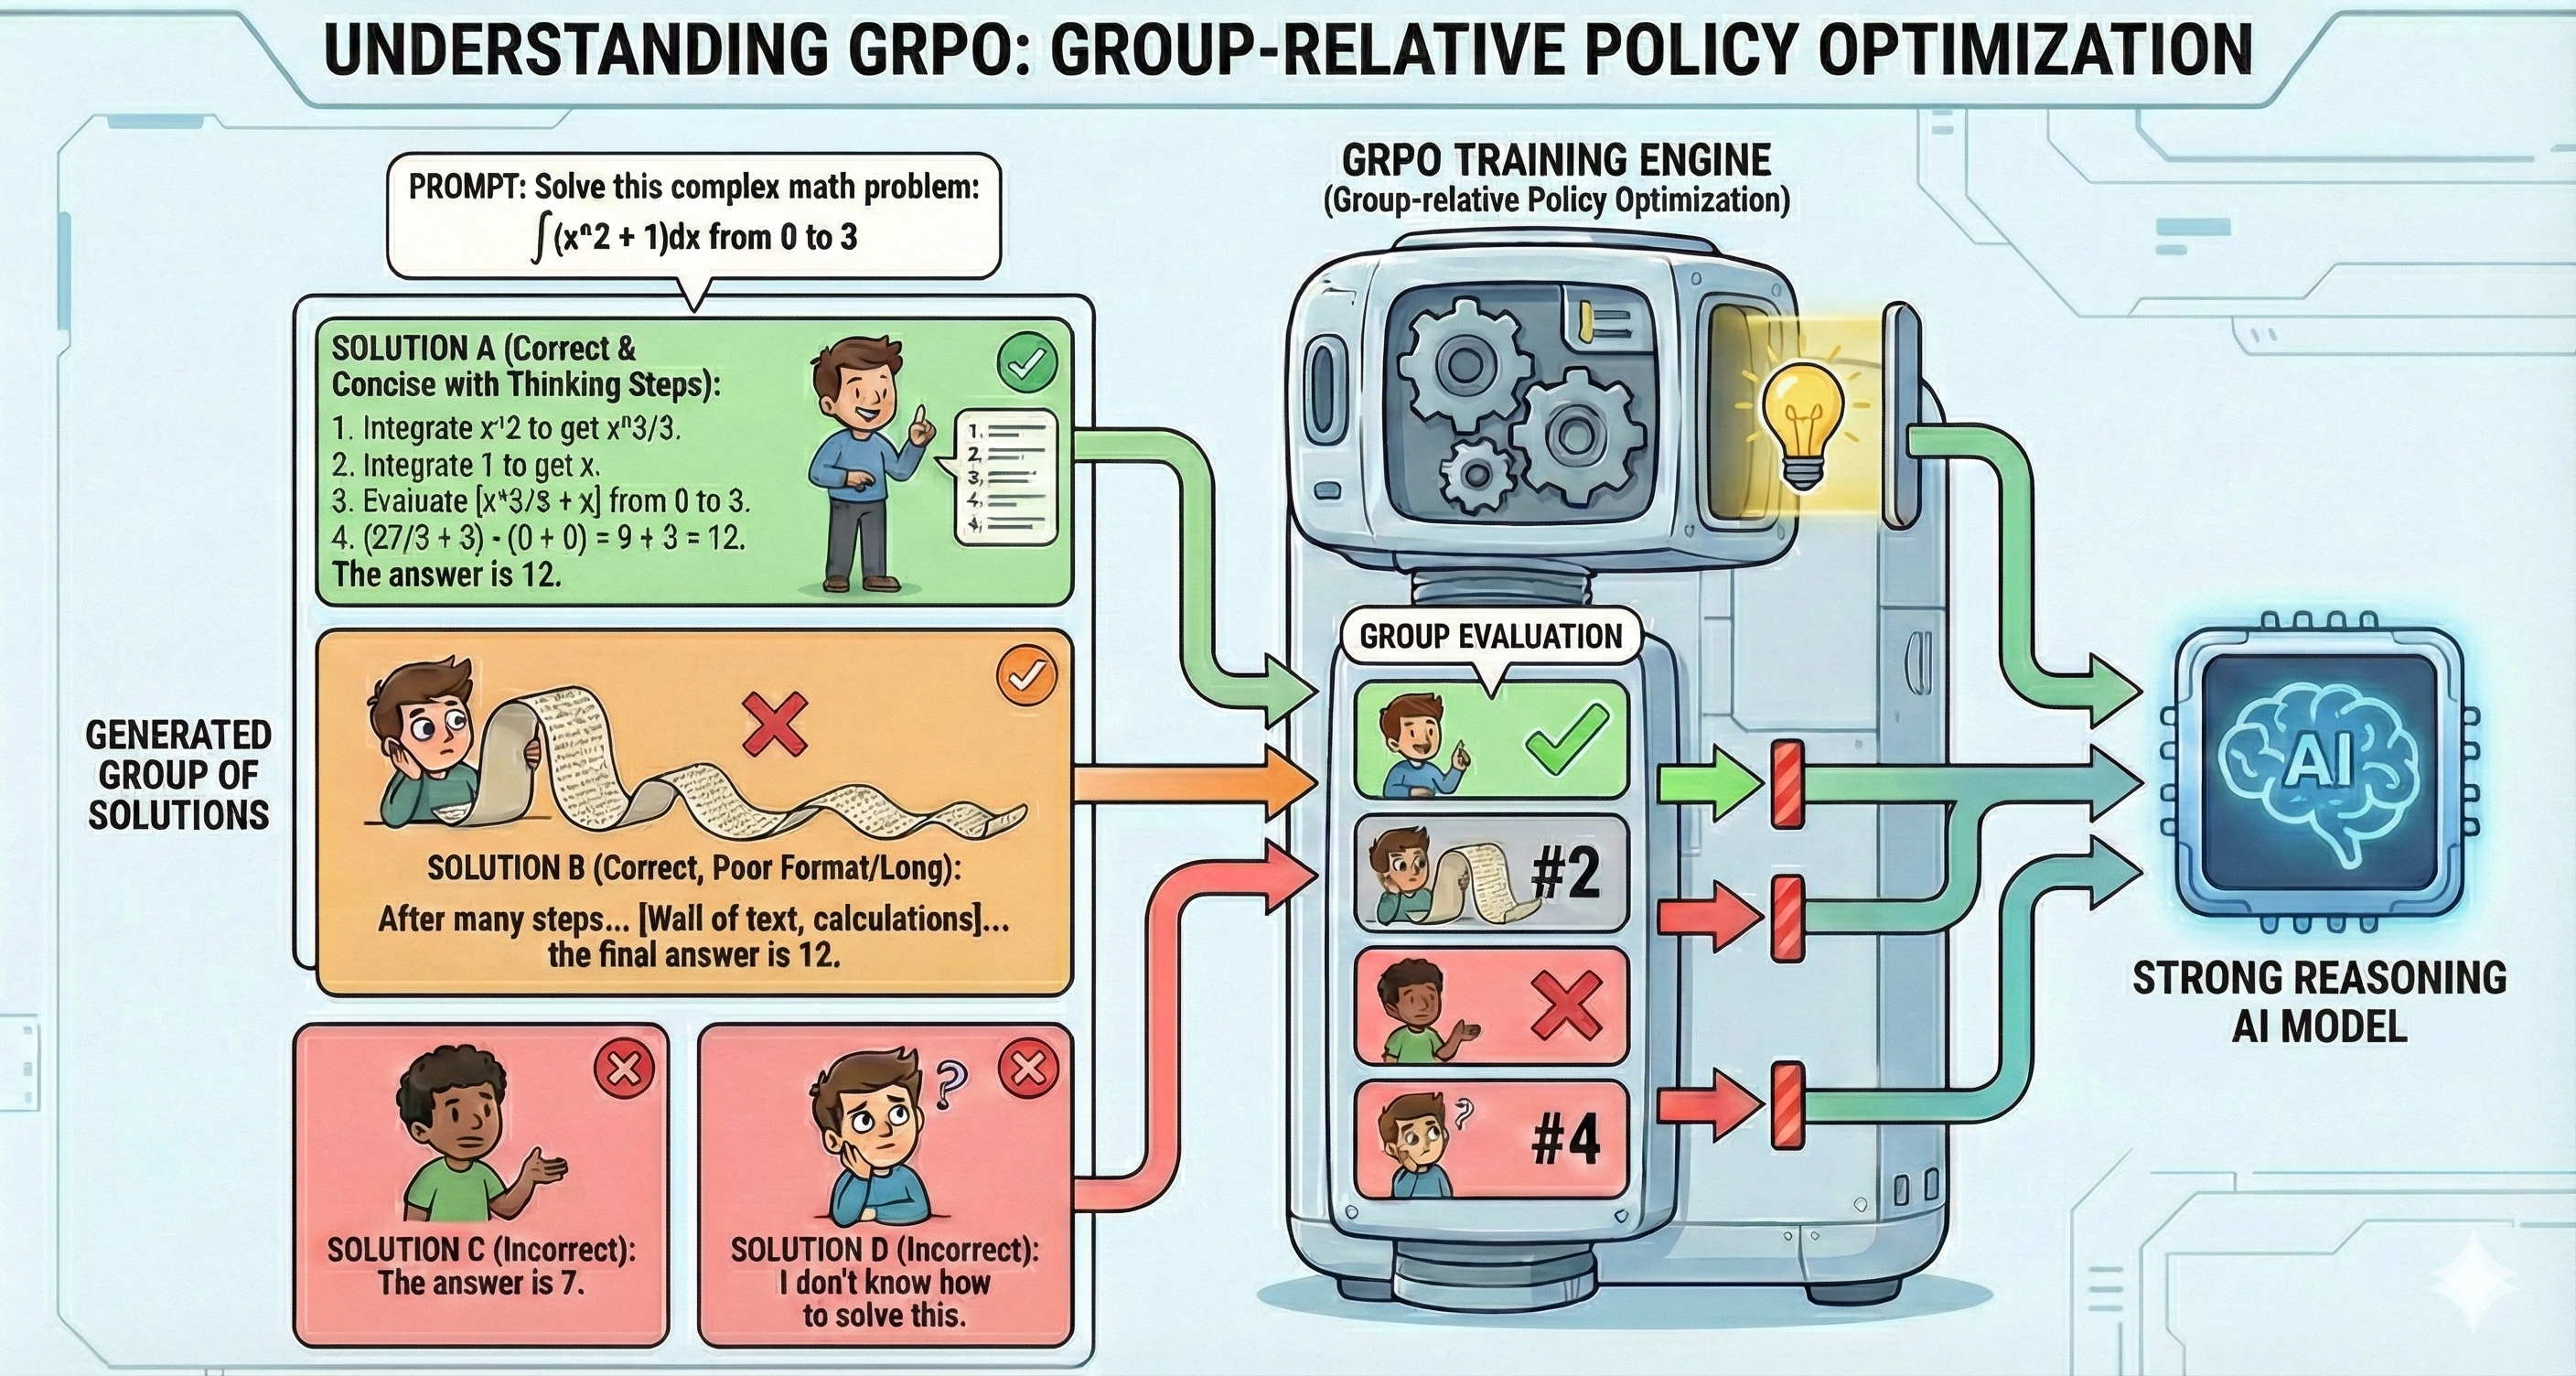
\includegraphics[width=0.75\textwidth]{figures/Gemini_Generated_Image_IllustrationGRPO.png}
        \caption{GRPO Illustration\footnotemark.}
    \end{figure}
    \footnotetext{\tiny Image generated by Nano Banana Pro.}
\end{frame}

% Slide 5: How GRPO Works (The Math)
\begin{frame}{The Mechanics of GRPO}
    \begin{itemize}
        \item \textbf{Step 1: Sampling.} For a prompt $q$, sample a group of $G$ outputs $\{o_1, o_2, ..., o_G\}$ from the old policy $\pi_{\theta_{old}}$.
        \item \textbf{Step 2: Scoring.} Compute rewards $r_i$ for each output using the verifier/checker.
        \item \textbf{Step 3: Advantage Calculation.} Instead of a value model $V(s)$, use the group average as the baseline:
        \[
            A_i = \frac{r_i - \text{mean}(\{r_1...r_G\})}{\text{std}(\{r_1...r_G\}) + \epsilon}
        \]
        \item \textbf{Step 4: Optimization.} Maximize the objective:
        \[
            \mathcal{L}_{GRPO} = \frac{1}{G} \sum_{i=1}^{G} \min \left( \frac{\pi_\theta(o_i|q)}{\pi_{\theta_{old}}(o_i|q)} A_i, \text{clip}(\frac{\pi_\theta(o_i|q)}{\pi_{\theta_{old}}(o_i|q)}, 1-\epsilon, 1+\epsilon) A_i \right) - \beta \mathbb{D}_{KL}
        \]
    \end{itemize}
\end{frame}

% Slide 5
\begin{frame}{Group Relative Policy Optimization (GRPO)}
    \begin{figure}
        \centering
        % "width=0.8\textwidth" scales the image to 80% of the text width
        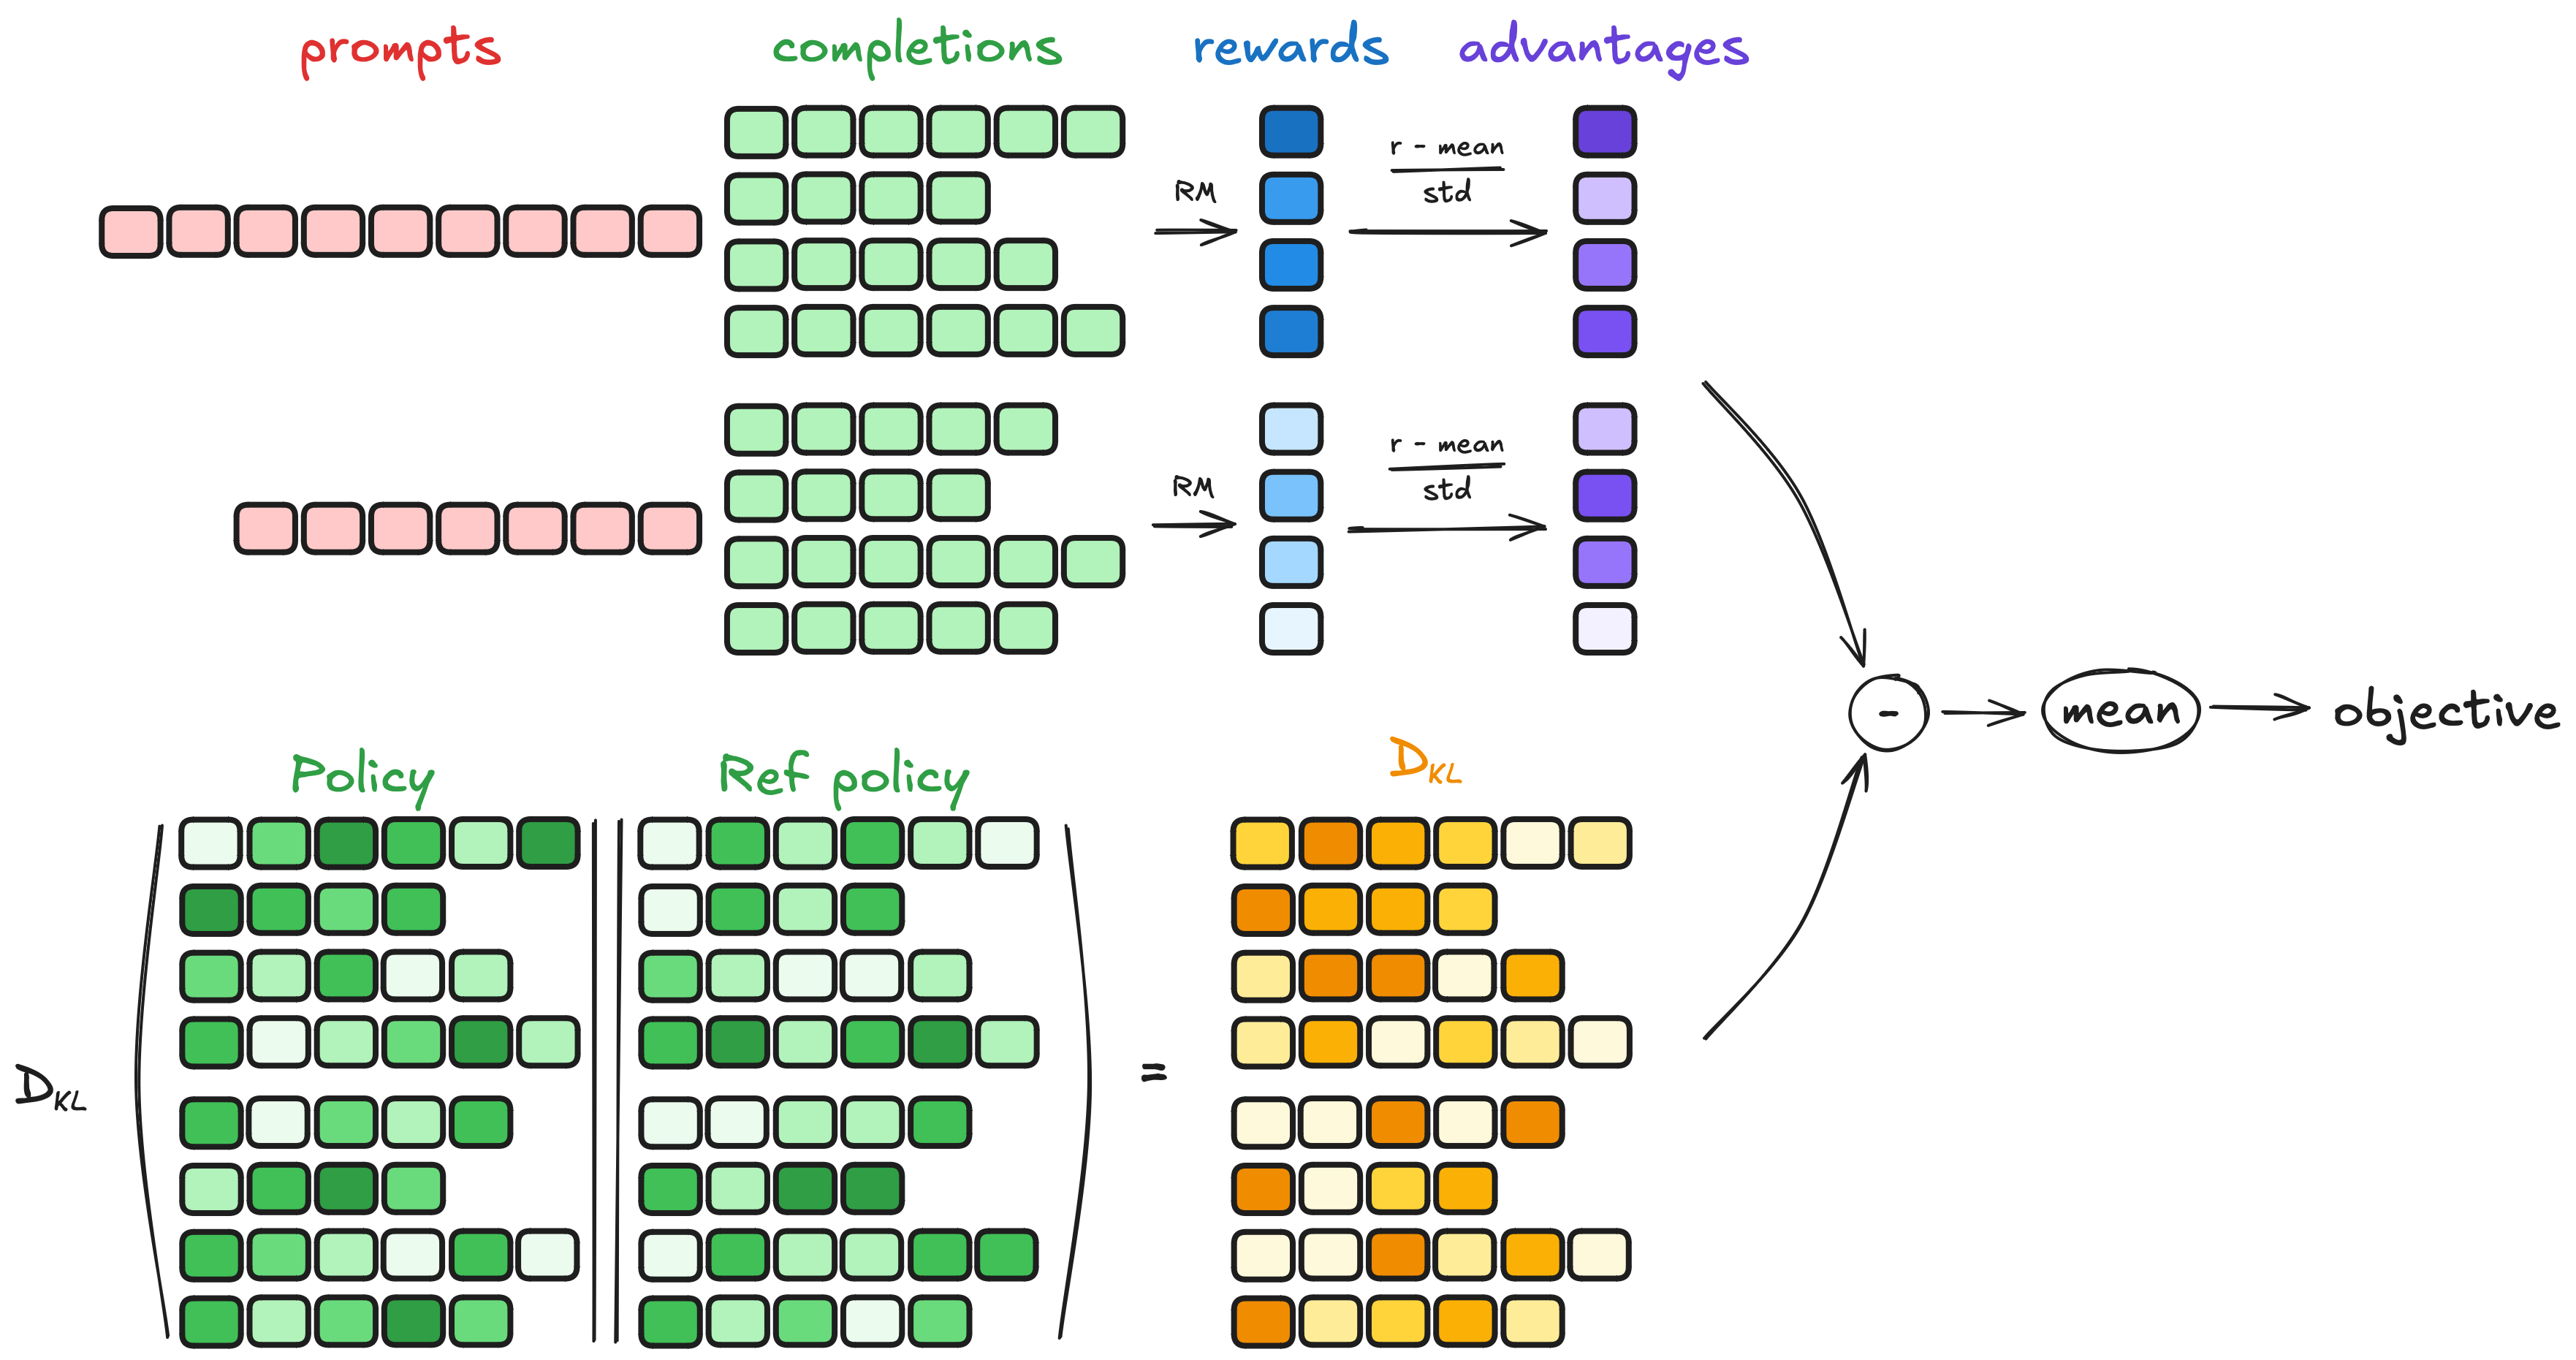
\includegraphics[width=0.75\textwidth]{figures/grpo_visual.png}
        \caption{GRPO Explanation\footnotemark.}
    \end{figure}
    \footnotetext{\tiny https://huggingface.co/docs/trl/main/en/grpo_trainer}
\end{frame}

% Slide 6: Why GRPO for Reasoning?
\begin{frame}{Why GRPO over PPO/DPO for Reasoning?}
    \begin{itemize}
        \item \textbf{No Value Model Needed:} PPO requires training a separate Value Model (critic) which is expensive and unstable. GRPO uses the group average as the baseline.
        \item \textbf{No Reference Model Forward Pass (Training):} GRPO estimates the KL divergence effectively without always needing a full forward pass of the reference model at every step (depending on implementation).
        \item \textbf{Comparison is Key:} By generating multiple attempts ($G=16$ or $G=64$), the model learns "Output A is better than Output B" directly from the variance in the group.
    \end{itemize}
\end{frame}

% Slide 7: Implementing the GRPO Trainer (The "Aha" Moment)
\begin{frame}{Implementing the GRPO Trainer}
    \begin{itemize}
        \item \textbf{Input Data:} A dataset of prompts $q$ and ground truth answers $y$ (e.g., GSM8K, MATH).
        \item \textbf{The Loop:}
    \end{itemize}
    \begin{algorithm}[H]
    \begin{algorithmic}[1]
    \State Sample batch of prompts $Q$
    \State Generate $G$ completions for each $q \in Q$
    \State Extract answers and run \texttt{verify\_reward(answer, truth)}
    \State Compute Advantages $A_i$ using Group Normalization
    \State Compute Loss and Update $\pi_\theta$
    \end{algorithmic}
    \caption{GRPO Training Loop}
    \end{algorithm}
\end{frame}

% Slide 8: The Code - Loss Calculation
\begin{frame}[fragile]{The Code: GRPO Loss Implementation}
\begin{lstlisting}[language=Python, basicstyle=\tiny\ttfamily]
def grpo_loss(self, model, batch):
    # 1. Forward pass (Policy & Reference)
    logits = model(batch['input_ids'])
    ref_logits = self.ref_model(batch['input_ids']) # Needed for KL
    
    # 2. Log probabilities & KL Divergence
    logprobs = compute_logprobs(logits, batch['labels'])
    ref_logprobs = compute_logprobs(ref_logits, batch['labels'])
    kl = torch.exp(ref_logprobs - logprobs) - (ref_logprobs - logprobs) - 1 # Approx KL

    # 3. Advantages (Group Normalized)
    # rewards shape: [batch_size, group_size] -> gathered from environment
    rewards = batch['rewards'] 
    mean, std = rewards.mean(dim=1, keepdim=True), rewards.std(dim=1, keepdim=True)
    advantages = (rewards - mean) / (std + 1e-8)
    
    # 4. PPO-style Clipped Loss + KL Penalty
    ratio = torch.exp(logprobs - batch['old_logprobs'])
    surr1 = ratio * advantages
    surr2 = torch.clamp(ratio, 1-eps, 1+eps) * advantages
    
    # Final Loss: Maximize Reward - Beta * KL Divergence
    loss = -torch.min(surr1, surr2).mean() + self.beta * kl.mean()
    
    return loss
\end{lstlisting}
\end{frame}

% Slide 9: "Aha-Moment" - What to expect?
\begin{frame}{The "Aha-Moment" in Training}
    \begin{itemize}
        \item \textbf{Early Stage:} The model tries to guess the answer directly. Low reward.
        \item \textbf{Mid Stage:} The model starts outputting longer chains of thought.
        \item \textbf{Format Adherence:} The model learns strict formatting because the verifier penalizes bad formats.
        \item \textbf{The "Aha":} You will observe the \textbf{length} of the response increase as accuracy increases. The model "learns" that thinking longer leads to higher verified rewards.
    \end{itemize}
    % \begin{center}
    %     \textit{"Diversity-Driven Optimization Elicits Large-Model Reasoning Ability"}
    % \end{center}
\end{frame}

% Slide 7
\begin{frame}{Training GRPO in Practice}
\begin{itemize}
  \item Run this \href{https://colab.research.google.com/drive/1hydSFeV8hpTleZTp5EwpoDCjrqRp8JQ7?usp=sharing}{Google Colab Notebook\footnotemark}.
  \item Before start training, you can enroll in the Google Colab Pro by going to https://colab.research.google.com/signup and select 'No cost for students and educators'. Then enter your information to activate the free offer of Colab Pro. This will give you access to strong GPU such as A100 which speeds up the training of LLMs.
\end{itemize}
\footnotetext{\tiny https://colab.research.google.com/drive/1hydSFeV8hpTleZTp5EwpoDCjrqRp8JQ7?usp=sharing}
\end{frame}

% Slide 8
\begin{frame}{GRPO Training Curves}

\begin{figure}
    \centering
    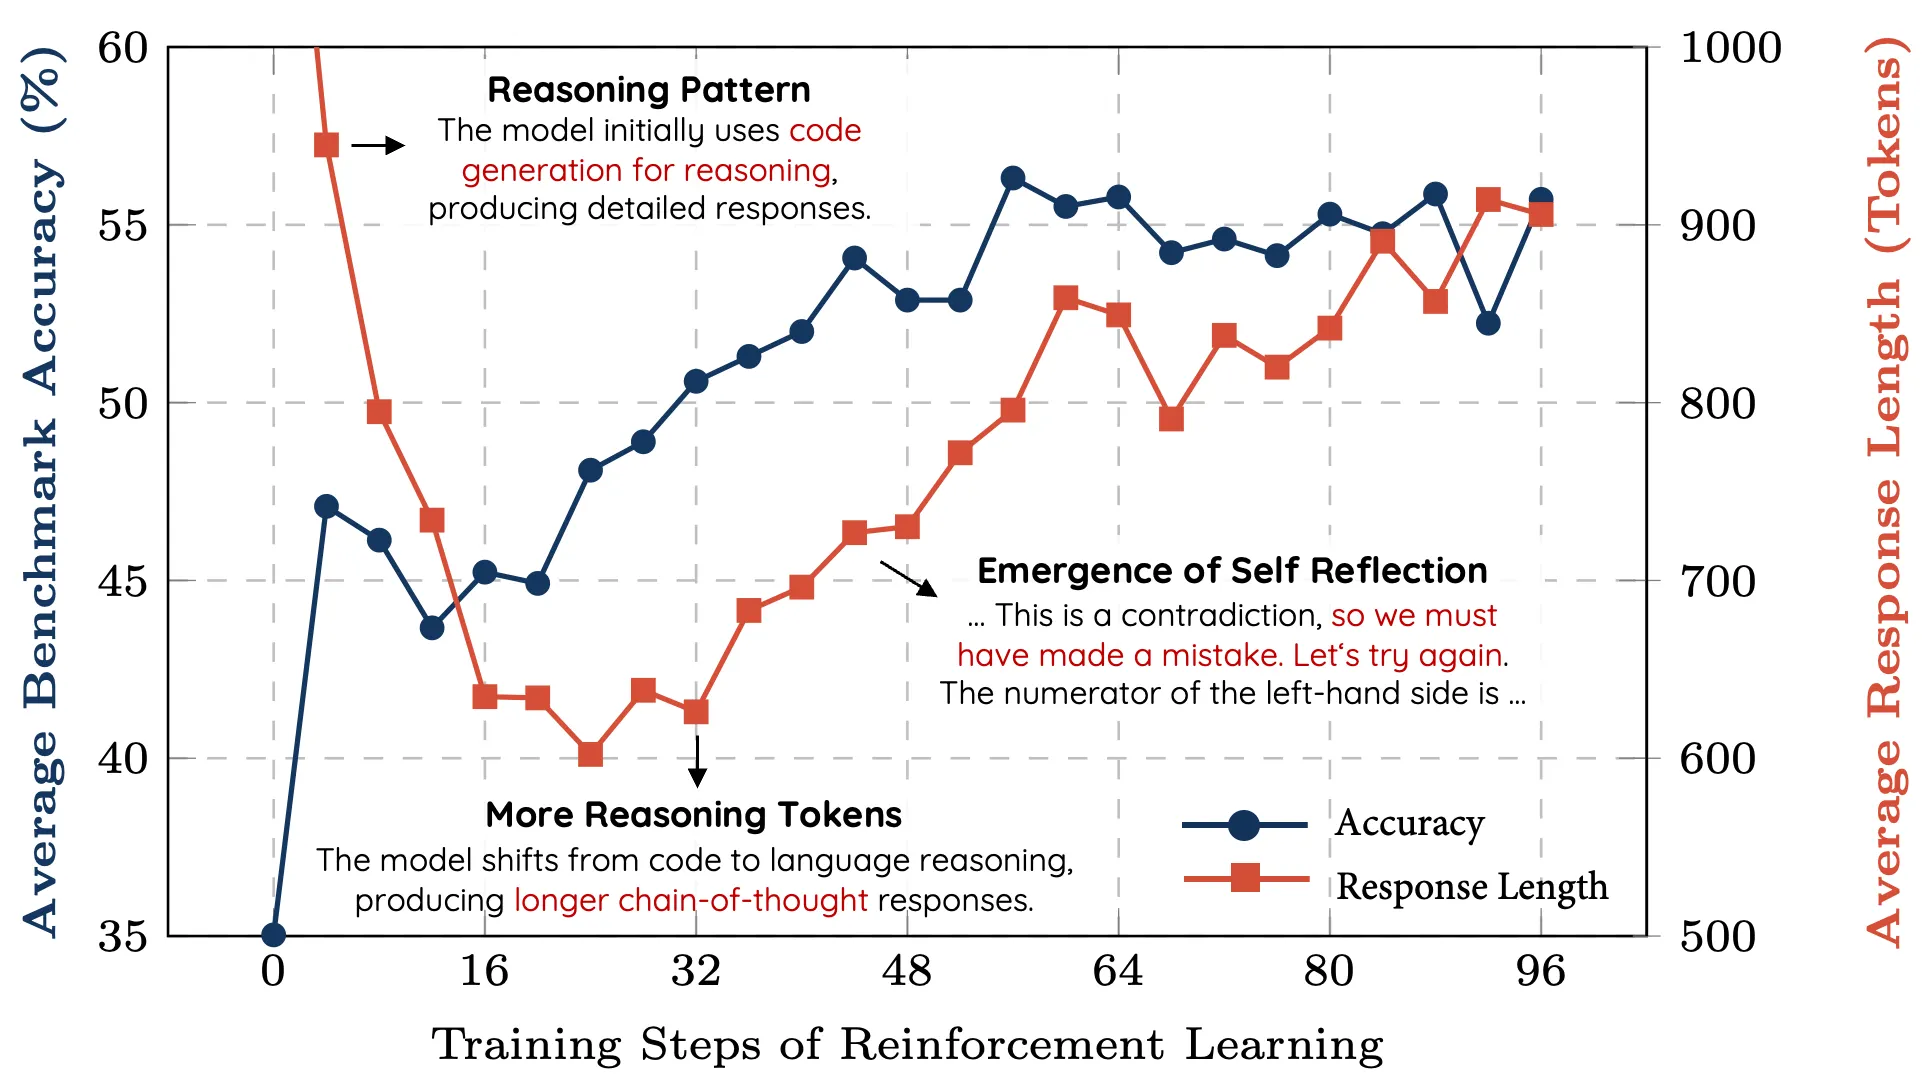
\includegraphics[width=0.75\textwidth]{figures/image_1.png}
    \caption{Examplar Training Curve.}
\end{figure}
% \footnotetext{\tiny Image borrowed from the https://hkust-nlp.notion.site/simplerl-reason.}

\end{frame}

% % Slide 3
% \begin{frame}{How to implement the DPOTrainer?}
% \begin{columns}
%     \begin{column}{0.5\textwidth}
%         \begin{itemize}
%         \item First compute the current policy's logits (i.e., vocab probability at each position that has label) for both the chosen and reject response.
%         \item Then compute the current policy's logp (i.e., only compute the probability of the target token). The logp is sumed or averaged over the whole response $y_w$ and $y_l$).
%         \item Compute the reference policy's logp. 
%         \end{itemize}
%     \end{column}
%     \begin{column}{0.5\textwidth}
%         \begin{figure}
%           \centering
%           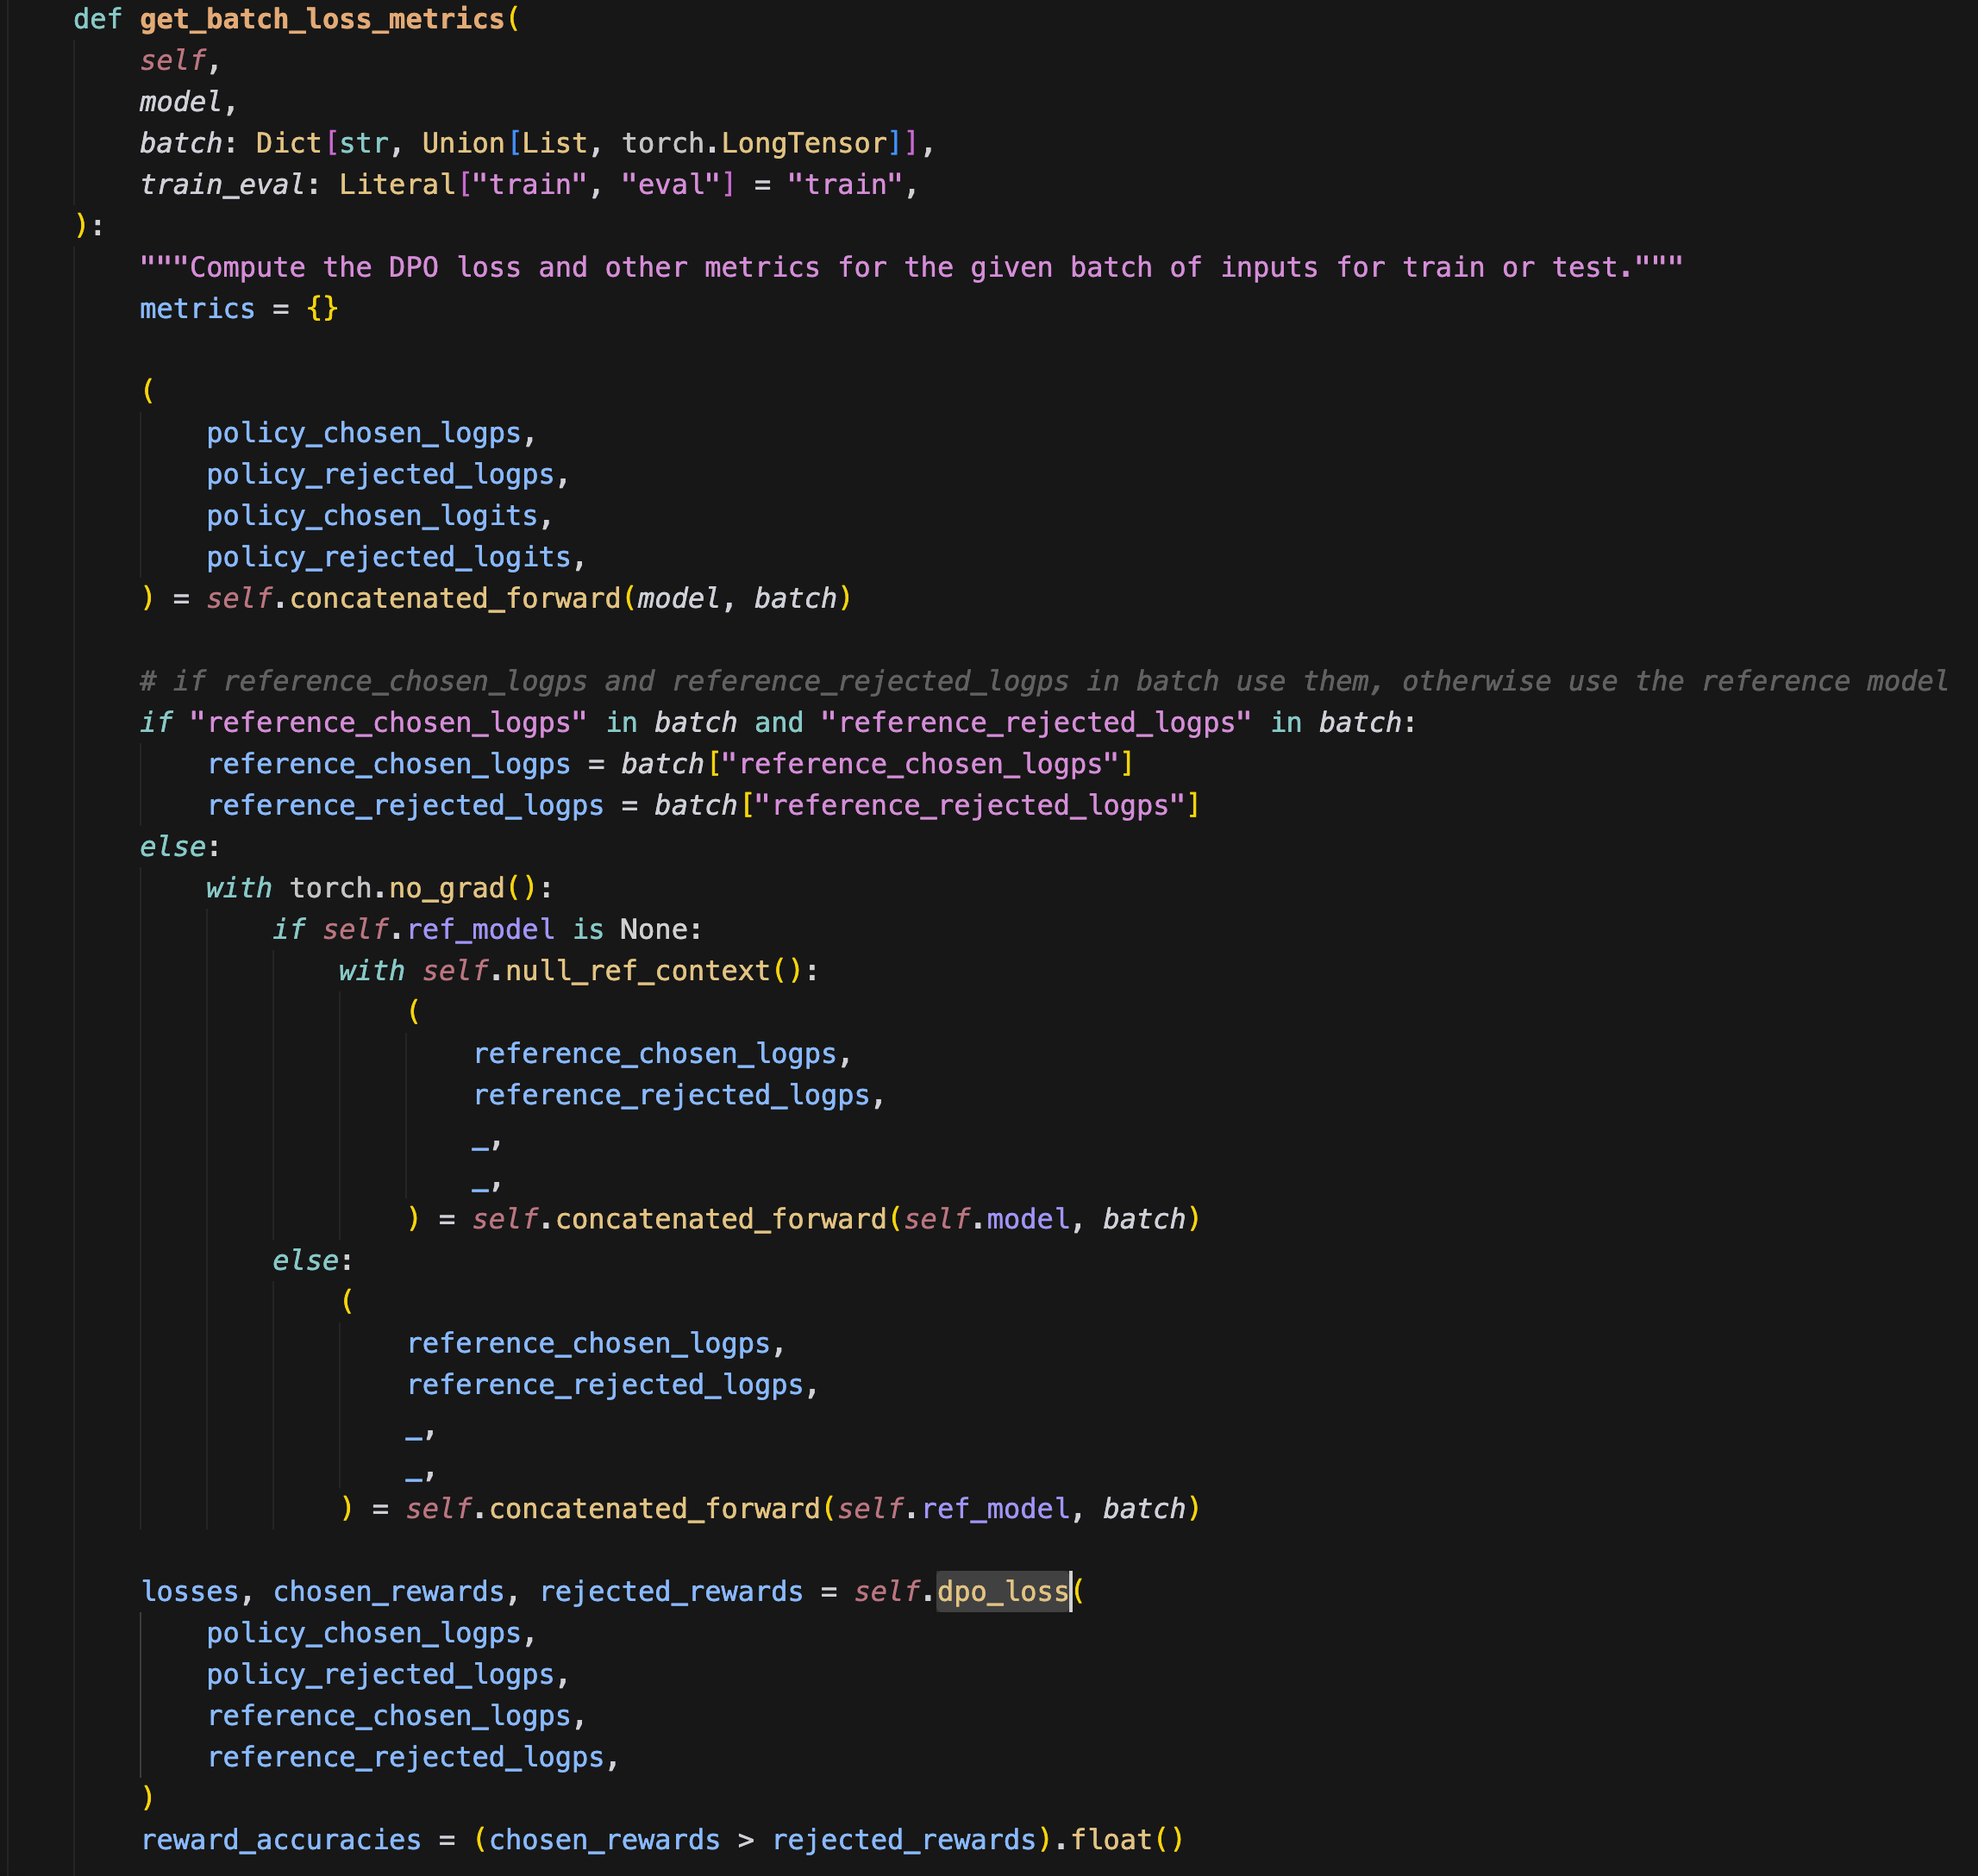
\includegraphics[width=\linewidth]{figures/Loss.png}
%           \label{fig:dpotrainer_loss}
%         \end{figure}
%     \end{column}
% \end{columns}
% \end{frame}

% \begin{frame}{How to implement the DPOTrainer?}
% \begin{columns}
%     \begin{column}{0.5\textwidth}
%         \begin{itemize}
%         \item First compute the logratio for both the current policy and reference model.
%         \item Then the distance between these two logratios.
%         \item Finally, based on different types of the loss function, we can use sigmoid or hinge loss to compute the final loss.
%         \end{itemize}
%     \end{column}
%     \begin{column}{0.5\textwidth}
%         \begin{figure}
%           \centering
%           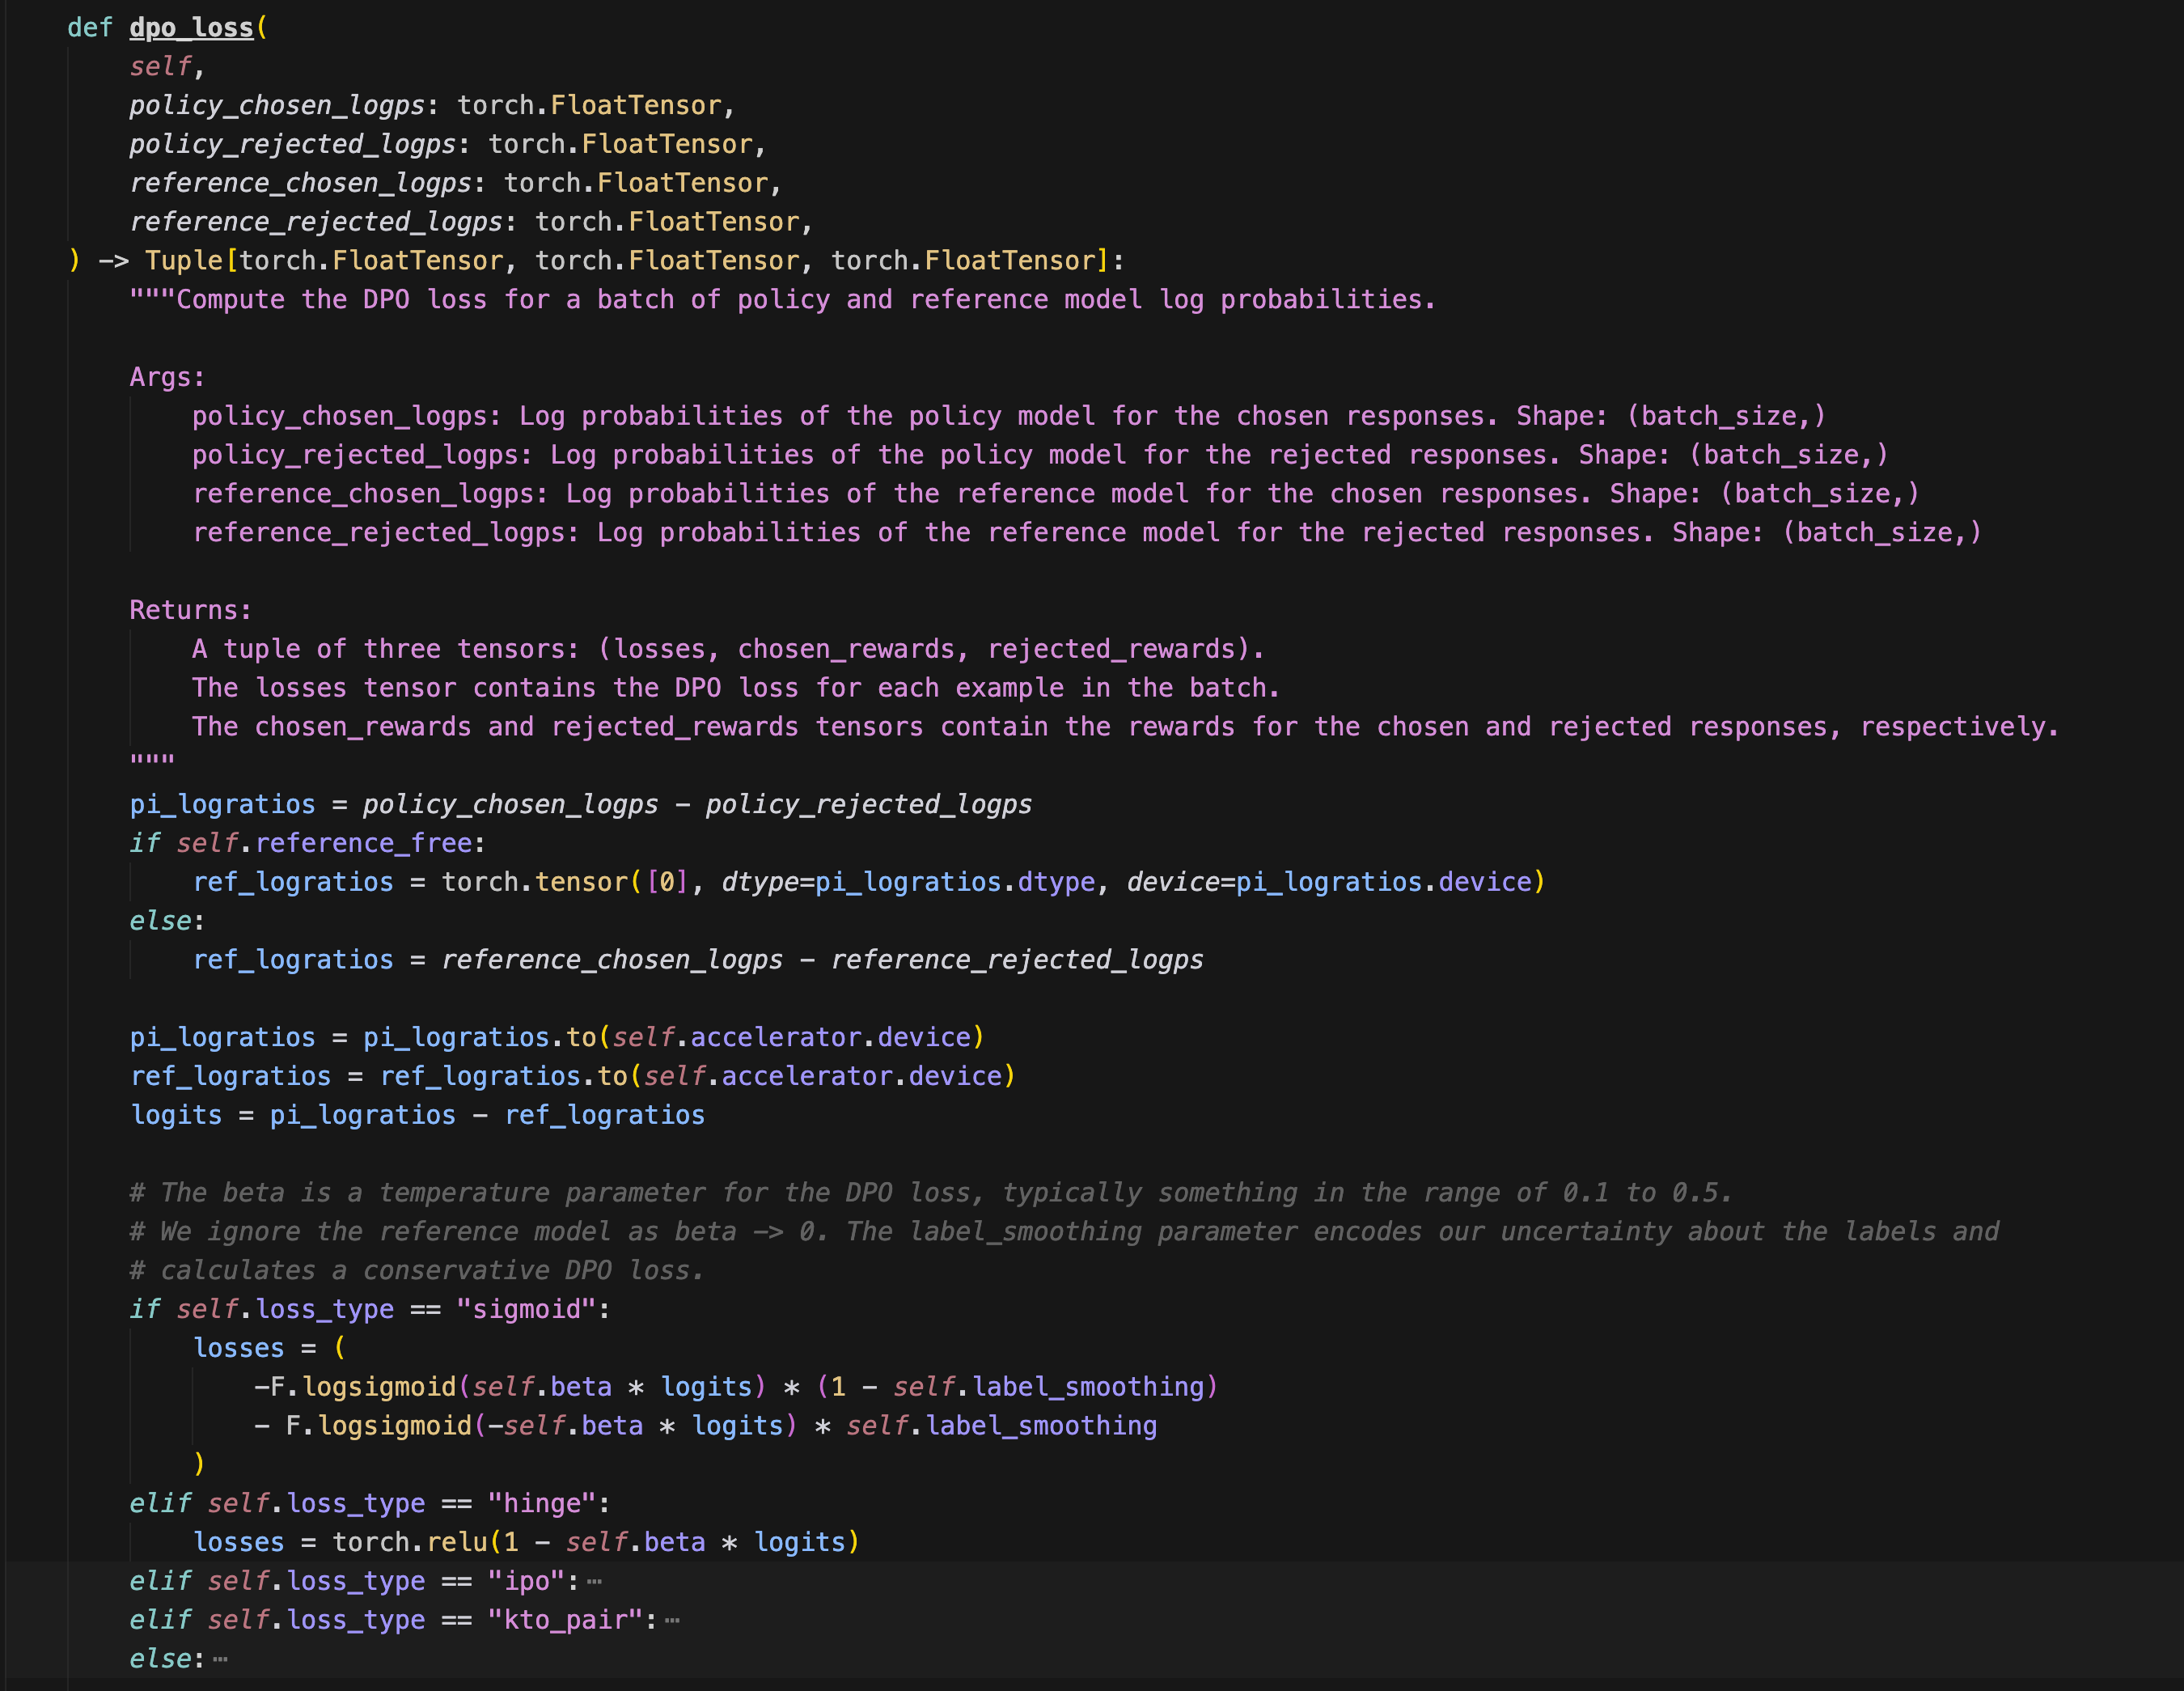
\includegraphics[width=\linewidth]{figures/DPO Loss.png}
%         \end{figure}
%         \label{fig:dpo_loss}
%     \end{column}
% \end{columns}
% \end{frame}


% Slide 10
\begin{frame}{Thanks!}
\centering
Questions?
\end{frame}

% % References slide
% \begin{frame}[allowframebreaks]{References}
% \printbibliography
% \end{frame}

\end{document}
